% arara: xelatex: {shell: yes}
%% arara: biber
%% arara: xelatex: {shell: yes}
%% arara: xelatex: {shell: yes}


% Здесь мы держим компромисс между красотой и легкостью включения новых людей в процесс создания.
% Поэтому не используем пакеты, которые требуют возни с установкой и настройкой.
% Например, используем listings вместо minted.
% Пакет minted требует настроенного питона и связки латех-питон. 
% Вместо arara используем классический latexmk. 


% TODO: по окончании курса переставить 6.8 между 6.5 и 6.6, тк 6.8 — это 6.5 с другими цифрами.
% TODO: прикольные или красивые картинки в начале каждого раздела


%!TeX cleanPatterns = $OUTDIR/$JOB!($OUTEXT|.synctex.gz|.tex|.pdf), /$OUTDIR/_minted-$JOB/
\documentclass[12pt, a4paper]{article}

% utf8 is the preferred encoding

 % this magic is to solve problem that appeared after update of texlive 2018 to texlive 2020
 % https://tex.stackexchange.com/questions/511341/the-error-occurred-after-the-last-update
\makeatletter
\def\nobreak{\penalty\@M}
\makeatother

\usepackage{comment}

\usepackage{fontspec} % что-то про шрифты? % нужно ли загружать?

\usepackage{polyglossia} % русификация xelatex
\usepackage{csquotes}
\usepackage{wrapfig} % обтекание картинок
\usepackage{xparse} % для прикольных вероятностей


\setmainlanguage{russian}

% download "Linux Libertine" fonts:
% http://www.linuxlibertine.org/index.php?id=91&L=1
\setmainfont{Linux Libertine O} % or Helvetica, Arial, Cambria
% why do we need \newfontfamily:
% http://tex.stackexchange.com/questions/91507/
\newfontfamily{\cyrillicfonttt}{Linux Libertine O}

\newfontfamily\arabicfont[Script=Arabic]{Scheherazade New}


\usepackage{etoolbox} % provides \AtEndPreamble
% etoolbox causes wrong behavior of tocbasic
\AtEndPreamble{ % ради арабского написания Абу ибн-Сина
  \usepackage{arabxetex} 
 \let\textarabic\relax 
 \let\Arabic\relax 
\setotherlanguages{arabic, british, chinese}
}
% комбо из:
% https://tex.stackexchange.com/questions/501897
% https://tex.stackexchange.com/questions/392175/

\usepackage[nonewpage]{imakeidx} 
%\indexsetup{level=\section}
\indexsetup{level=\section,toclevel=section,noclearpage}
\makeindex[intoc,title={Модные хэштэги}] % [title=Модные хэштэги, intoc]
% TODO: лишняя пустая страница в printindex

\usepackage{etex} % расширение классического tex
% в частности позволяет подгружать гораздо больше пакетов, чем мы и займёмся далее

\usepackage{verbatim} % для многострочных комментариев
\usepackage{makeidx} % для создания предметных указателей

\usepackage{setspace}
\usepackage{amsmath, amsfonts, amssymb, amsthm}
\usepackage{mathrsfs} % sudo yum install texlive-rsfs
\usepackage{dsfont} % sudo yum install texlive-doublestroke
\usepackage{array, multicol, multirow, bigstrut} % sudo yum install texlive-multirow
\usepackage{indentfirst} % установка отступа в первом абзаце главы


\usepackage{bm}
\usepackage{bbm} % шрифт с двойными буквами
%\usepackage[perpage]{footmisc}

\usepackage{dcolumn} % центрирование по разделителю для apsrtable

% создание гиперссылок в pdf
\usepackage[unicode, colorlinks=true, urlcolor=blue, 
citecolor=blue, hyperindex, breaklinks]{hyperref}


\usepackage{microtype} % свешиваем пунктуацию
% теперь знаки пунктуации могут вылезать за правую границу текста, при этом текст выглядит ровнее


\usepackage{textcomp}  % Чтобы в формулах можно было русские буквы писать через \text{}

% размер листа бумаги
%\usepackage[paperwidth=145mm,paperheight=215mm,
%height=182mm,width=113mm,top=20mm,includefoot]%{geometry}
\usepackage[paper=a4paper, top=15mm, bottom=13.5mm, left=16.5mm, right=13.5mm, includefoot]{geometry}

\usepackage{xcolor}
\usepackage{framed} % для рамок и черты слева от минитеории, \leftbar

% \usepackage{float, longtable}
\usepackage{soulutf8}

\usepackage{enumitem} % дополнительные плюшки для списков
%  например \begin{enumerate}[resume] позволяет продолжить нумерацию в новом списке

\usepackage{mathtools}
\usepackage{cancel, xspace} % sudo yum install texlive-cancel


\usepackage{numprint} % sudo yum install texlive-numprint
\npthousandsep{,}\npthousandthpartsep{}\npdecimalsign{.}


% \usepackage{subfigure} % для создания нескольких рисунков внутри одного

\usepackage{tikz, pgfplots} % язык для рисования графики из latex'a
\pgfplotsset{compat=1.16}
% \usetikzlibrary{trees} % tikz-прибамбас для рисовки деревьев
\usepackage{tikz-qtree} % альтернативный tikz-прибамбас для рисовки деревьев
\usepackage{tkz-graph} % by dp for making prob trees
\usetikzlibrary{shapes.geometric, arrows, automata, trees} % tikz-прибамбас для рисовки стрелочек подлиннее



\tikzstyle{normal} = [rectangle, 
minimum width=3cm, 
minimum height=1cm, 
text centered, 
draw=black, 
fill=green!30]

\tikzstyle{decision} = [rectangle, 
minimum width=3cm, 
minimum height=1cm, 
text centered, 
draw=black, 
fill=green!30]

\tikzstyle{arrow} = [thick,->,>=stealth]




\usepackage{todonotes} % для вставки в документ заметок о том, что осталось сделать
% \todo{Здесь надо коэффициенты исправить}
% \missingfigure{Здесь будет Последний день Помпеи}
% \listoftodos — печатает все поставленные \todo'шки



\usepackage{booktabs} %  красивые таблицы
% заповеди из докупентации:
% 1. Не используйте вертикальные линни
% 2. Не используйте двойные линии
% 3. Единицы измерения - в шапку таблицы
% 4. Не сокращайте .1 вместо 0.1
% 5. Повторяющееся значение повторяйте, а не говорите "то же"

%\usepackage{physics} % не рекомендуют его использовать
% конфликтует много с кем, плохая реализация
% https://tex.stackexchange.com/questions/471532/alternatives-to-the-physics-package
\DeclareMathOperator{\bneck}{bneck}
\DeclarePairedDelimiter{\norm}{\lVert}{\rVert}
\DeclarePairedDelimiter{\abs}{\lvert}{\rvert}
\DeclarePairedDelimiter{\scalp}{\langle}{\rangle}



\usepackage{listings}
\lstset{%
basicstyle=\fontfamily{lmtt}\bfseries,
keywordstyle=\fontfamily{lmtt}\bfseries
}

\usepackage{answers}

\newenvironment{rus}{}{} % environment just prints the text
\newenvironment{eng}{}{}
\excludecomment{eng}



\usepackage[bibencoding=auto, backend=biber, sorting=none, style=alphabetic]{biblatex}

\addbibresource{probability_pro.bib}

\setcounter{tocdepth}{1} % в оглавление оставляем уровень 1

\usepackage[titles]{tocloft} % альтернатива tocbasic для настройки toc
% если нужен subfigure, то у tocloft можно добавить опцию subfigure
\renewcommand{\cftbeforesecskip}{0.7pt} % поправка интервала между строками для section в toc
\renewcommand{\cftsecdotsep}{\cftdotsep} % добавляем точечки

\AddEnumerateCounter{\asbuk}{\russian@alph}{щ} % для списков с русскими буквами
\setlist[enumerate, 1]{label=\asbuk*),ref=\asbuk*} % цифра рядом с enumerate = уровень нумерации


% transportation table 
% https://tex.stackexchange.com/questions/83713/how-to-make-a-transportation-tableau
\newcolumntype{C}{@{}c@{}}
\newcommand{\bottombox}[1]{\makebox[2em][r]{#1}\hspace*{\tabcolsep}\hspace*{2em}}%
\newcommand{\innerbox}[2]{%
    \begin{tabular}[b]{c|c}
       \rule{2em}{0pt}\rule[-2ex]{0pt}{5ex} & \makebox[0.9em]{\footnotesize{#2}} \\\cline{2-2}
       \multicolumn{2}{r}{{#1}\hspace*{1.5\tabcolsep}\hspace*{2em}\rule[-2ex]{0pt}{5ex}}
    \end{tabular}}
\renewcommand{\arraystretch}{1.25}





%%%%%%%%%%%%%%%%%%%%%%%  ПАРАМЕТРЫ  %%%%%%%%%%%%%%%%%%%%%%%%%%%%%%%%%%
\setstretch{1}                          % Межстрочный интервал
\flushbottom                            % Эта команда заставляет LaTeX чуть растягивать строки, чтобы получить идеально прямоугольную страницу
\righthyphenmin=2                       % Разрешение переноса двух и более символов
%\pagestyle{plain}                       % Нумерация страниц снизу по центру.
\widowpenalty=300                     % Небольшое наказание за вдовствующую строку (одна строка абзаца на этой странице, остальное — на следующей)
\clubpenalty=3000                     % Приличное наказание за сиротствующую строку (омерзительно висящая одинокая строка в начале страницы)
\setlength{\parindent}{1.5em}           % Красная строка.
%\captiondelim{. }
\setlength{\topsep}{0pt}
\emergencystretch=2em

% делаем короче интервал в списках
\setlength{\itemsep}{0pt}
\setlength{\parskip}{0pt}
\setlength{\parsep}{0pt}



\DeclareMathOperator{\card}{card}
\DeclareMathOperator{\sign}{sign}
\DeclareMathOperator{\sgn}{sign}

\DeclareMathOperator*{\argmin}{arg\,min}
\DeclareMathOperator*{\amn}{arg\,min}
\DeclareMathOperator*{\amx}{arg\,max}


\DeclareMathOperator{\Corr}{Corr}
\DeclareMathOperator{\sCorr}{sCorr}
\DeclareMathOperator{\sCov}{sCov}
\DeclareMathOperator{\sVar}{sVar}

%\DeclareMathOperator{\Cov}{Cov}
%\DeclareMathOperator{\Var}{Var}

\DeclareMathOperator*{\plim}{plim}
\DeclareMathOperator{\MSE}{MSE}
\DeclareMathOperator{\softmax}{softmax}
\DeclareMathOperator{\Med}{Med}


\DeclareMathOperator{\col}{col}
\DeclareMathOperator{\row}{row}


\let\P\relax
\DeclareMathOperator{\P}{\mathbb{P}}

% \newcommand{\P}{\mathbb{P}}



\newcommand{\oP}{o_{\operatorname{P}}} % вероятностное о-малое




\newcommand{\e}{\varepsilon}

\newcommand{\cN}{\mathcal{N}}

% вместо горизонтальной делаем косую черточку в нестрогих неравенствах
\renewcommand{\le}{\leqslant}
\renewcommand{\ge}{\geqslant}
\renewcommand{\leq}{\leqslant}
\renewcommand{\geq}{\geqslant}


\newcommand{\wv}{\textrm{word2vec}}
\newcommand{\hVar}{\widehat{\Var}}
\newcommand{\hCorr}{\widehat{\Corr}}
\newcommand{\hCov}{\widehat{\Cov}}


\newcommand{\PP}{\mathbb{P}}
\newcommand{\QQ}{\mathbb{Q}}
\newcommand{\RR}{\mathbb{R}}
\newcommand{\NN}{\mathbb{N}}
\newcommand{\ZZ}{\mathbb{Z}}
\newcommand{\cF}{\mathcal{F}}
\newcommand{\cB}{\mathcal{B}}
\newcommand{\cA}{\mathcal{A}}
\newcommand{\cH}{\mathcal{H}}


% dot of variable size, from
% https://tex.stackexchange.com/questions/389238/is-there-a-black-dot-symbol-that-i-can-use
\newcommand\vardot[1][.4]{\mathbin{\vcenter{\hbox{\scalebox{#1}{$\bullet$}}}}}
% dot above equality sign for Newton style
%\renewcommand{\doteq}{\mathrel{\overset{\vardot}{=}}}
\renewcommand{\doteq}{\mathrel{\overset{\lim}{=}}}



% from Blitzstein


\newcommand{\dBern}{\mathrm{Bern}}
\newcommand{\dPois}{\mathrm{Pois}}
\newcommand{\dBin}{\mathrm{Bin}}
\newcommand{\dMult}{\mathrm{Mult}}
\newcommand{\dGeom}{\mathrm{Geom}}
\newcommand{\dNHGeom}{\mathrm{NHGeom}}
\newcommand{\dHGeom}{\mathrm{HGeom}}
\newcommand{\dDUnif}{\mathrm{DUnif}}
\newcommand{\dFS}{\mathrm{FS}}
\newcommand{\dNBin}{\mathrm{NBin}}

\newcommand{\dTri}{\mathrm{Triangle}}
\newcommand{\dUnif}{\mathrm{Unif}}
\newcommand{\dU}{\mathrm{U}}
\newcommand{\dCauchy}{\mathrm{Cauchy}}
\newcommand{\dN}{\mathcal{N}}
\newcommand{\dLN}{\mathcal{LN}}
\newcommand{\dExpo}{\mathrm{Expo}} % o is probably great to avoid confusion with exp function
\newcommand{\dExp}{\dExpo}
\newcommand{\dBeta}{\mathrm{Beta}}
\newcommand{\dGamma}{\mathrm{Gamma}}
\newcommand{\dWei}{\mathrm{Wei}}
\newcommand{\dLogistic}{\mathrm{Logistic}}
\newcommand{\dRayleigh}{\mathrm{Rayleigh}}
\newcommand{\dPareto}{\mathrm{Pareto}}


\newcommand{\addtag}[1]{\index{#1}}

\DeclareMathOperator{\Convex}{Convex}
\DeclareMathOperator{\hull}{\Convex}
\DeclareMathOperator{\Hull}{Hull}
\DeclareMathOperator{\Span}{Span}
\DeclareMathOperator{\cone}{Cone}
\DeclareMathOperator{\degree}{degree}
\DeclareMathOperator{\closeness}{closeness}
\DeclareMathOperator{\betweenness}{betweenness}


\newcommand{\chinesetext}[1]{\setmainfont{Source Han Sans CN}
#1
\setmainfont{Linux Libertine O}}



% hack from
% https://tex.stackexchange.com/questions/14501/making-footnote-work-in-leftbar-environment/
% does not work with hyperref?
% \input{footnote-in-leftbar.tex}

\title{Заметки к семинарам по методам оптимальных решений}
\author{\url{https://github.com/bdemeshev/optimal-solution-pro} \\
зеркало: \url{https://gitlab.com/bdemeshev/optimal-solution-pro}}
\date{\today \\
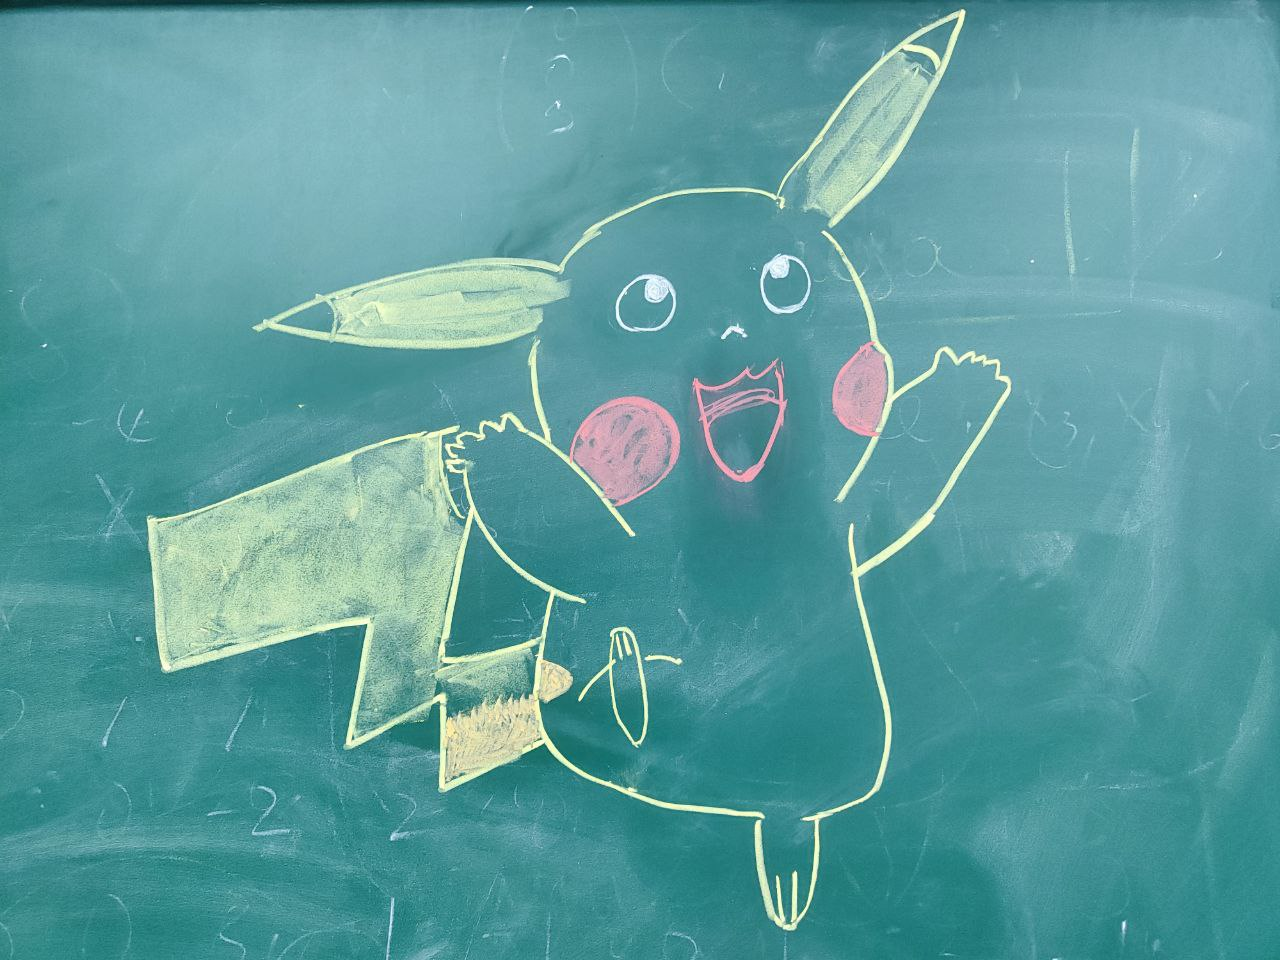
\includegraphics[height=10cm]{picachu.jpg} \\
\chinesetext{皮卡丘} } % 乒乓


%\newtheorem{problem}{Задача}
%\numberwithin{problem}{section}

\Newassociation{sol}{solution}{solution_file}
% sol — имя окружения внутри задач
% solution — имя окружения внутри solution_file
% solution_file — имя файла в который будет идти запись решений
% можно изменить далее по ходу
\Opensolutionfile{solution_file}[all_solutions]
% в квадратных скобках фактическое имя файла



% магия для автоматических гиперссылок задача-решение
\newlist{myenum}{enumerate}{3}
% \newcounter{problem}[chapter] % нумерация задач внутри глав
\newcounter{problem}[section]

\newenvironment{problem}%
{%
\refstepcounter{problem}%
%  hyperlink to solution
     \hypertarget{problem:{\thesection.\theproblem}}{} % нумерация внутри глав
     % \hypertarget{problem:{\theproblem}}{}
     \Writetofile{solution_file}{\protect\hypertarget{soln:\thesection.\theproblem}{}}
     %\Writetofile{solution_file}{\protect\hypertarget{soln:\theproblem}{}}
     \begin{myenum}[label=\bfseries\protect\hyperlink{soln:\thesection.\theproblem}{\thesection.\theproblem},ref=\thesection.\theproblem]
     % \begin{myenum}[label=\bfseries\protect\hyperlink{soln:\theproblem}{\theproblem},ref=\theproblem]
     \item%
    }%
    {%
    \end{myenum}}
% для гиперссылок обратно надо переопределять окружение
% это происходит непосредственно перед подключением файла с решениями





\begin{document}

\maketitle % ставим сюда название, автора и время создания


\newpage
\tableofcontents{}

\newpage

При везении подсказку, ответ или решение можно найти, кликнув по номеру задачи. 

% Если \url{github.com} не открывается, можно заменить его на \url{gitlab.com}.

Подробная книжка Фергюсона, \cite{ferguson2010lpintro}.
Слайды к оксфордскому курсу, \cite{law2010lpnotes}.

Обсуждение интуиции за двойственными задачами, \cite{223235}.

Слайды по алгоритмам Кляйнберга и Тардос, \cite{kleinberg2014algo}.



\section{Картинки на плоскости}

\begin{leftbar}
\noindent
Линейная оболочка (linear span):
\[
  \Span(v_1, v_2, v_3) = \{x_1 v_1 + x_2 v_2 + x_3 v_3 \mid x_1 \in \RR, x_2 \in \RR, x_3 \in \RR \}
\]
Конус (cone):
\[
  \cone(v_1, v_2, v_3) = \{x_1 v_1 + x_2 v_2 + x_3 v_3 \mid x_1 \geq 0, x_2 \geq 0, x_3 \geq 0 \}
\]
Выпуклая линейная оболочка (convex linear hull):
\[
  \Hull(v_1, v_2, v_3) = \Convex(v_1, v_2, v_3) = \left\{x_1 v_1 + x_2 v_2 + x_3 v_3 \mid x_1 \geq 0, x_2 \geq 0, x_3 \geq 0, \sum x_i = 1 \right\}
\]
\end{leftbar}


\begin{problem}
  Рассмотрим точки на плоскости, $A = (0, 0)$, $B = (5, 3)$ и $C = (5, -3)$.
  
  \begin{enumerate}
    \item Нарисуйте точки $0.5 B + 0.5 C$, $0.9 A + 0.1 B$, $3 B - 2 C$.
    \item Нарисуйте точки $\frac{1}{3}A + \frac{1}{3}B + \frac{1}{3}C$, $0.1 A + 0.45 B + 0.45 C$, $0.9A + 0.05B + 0.05C$.
  \end{enumerate}
  
  \begin{sol}
  
  \end{sol}
  \end{problem}
  


\begin{problem}
Рассмотрим точки на плоскости, $A = (1, 2)$, $B = (3, 4)$ и $C = (5, 1)$.

\begin{enumerate}
  \item Нарисуйте $\hull(A, B)$, $\hull(A, B, C)$.
  \item Нарисуйте $\cone(A)$, $\cone(A, B)$, $\cone(A, B, C)$.
  \item Нарисуйте $\Span(A)$, $\Span(A, B)$.
  \item Нарисуйте $A + \Span(B)$, $\cone(A) + \cone(B)$.
  \item Нарисуйте $\hull(A, B) + \cone(C)$, $\hull(A) + \cone(B, C)$, $\hull(A, C) + \cone(B, C)$.
\end{enumerate}

\begin{sol}

\end{sol}
\end{problem}


\begin{problem}
Рассмотрим точки на плоскости $A = (1, 2)$, $B = (5, 2)$, $C = (1, 4)$, $D = (5, 4)$.
\begin{enumerate}
  \item Запишите $E = (1, 3)$ как выпуклую линейную комбинацию точек $A$, $B$, $C$ и $D$.
  \item Запишите $F = (3, 3)$ как выпуклую линейную комбинацию точек $A$, $B$, $C$ и $D$ всеми возможными способами.
  \item Можно ли записать $G = (6, 3)$ как выпуклую линейную комбинацию точек $A$, $B$, $C$ и $D$?
  \item Сколькими способами можно записать $H = (4, 3)$ как выпуклую линейную комбинацию $A$, $B$, $C$ и $D$?
  \item Сколькими способами можно записать $I = (4, 3)$ как выпуклую линейную комбинацию $A$, $B$ и $D$? 
  \item Сколькими способами можно записать $J = (4, 2)$ как выпуклую линейную комбинацию $A$, $B$, $C$ и $D$?
  \item Сколькими способами можно записать $K = (4, 2)$ как выпуклую линейную комбинацию $A$, $C$ и $D$?
\end{enumerate}

\begin{sol}
\begin{enumerate}
  \item $E = 0.5 A + 0B +  0.5 C + 0D$
  \item Например, $F = 0A + 0.5B + 0.5 C + 0D = 0.5A + 0B + 0C + 0.5D = 0.25A + 0.25B + 0.25C + 0.25D$.
  Для нахождения всех способов надо решить систему:
  \[
  \alpha A + \beta B + \gamma C + \delta D = E \\
  \alpha  + \beta  + \gamma  + \delta  = 1
  \]
  \[
\left(\begin{array}{cccc|c}
    1 & 5 & 1& 5 & 3 \\
    2 & 2 & 4 & 4 & 3 \\
    1 & 1 & 1 & 1 & 1 
\end{array}\right)    \to \ldots \to 
\left(\begin{array}{cccc|c}
    0 & 1 & 0 & 1 & 1/2 \\
    0 & 0 & 1 & 1 & 1/2 \\
    1 & 0 & 0 & -1 & 0 
\end{array}\right)
\]
  Система имеет бесконечное количество решений.

  Все способы, $F = \alpha A + (0.5 - \alpha) B + (0.5 - \alpha)C + \alpha D$, где $\alpha \in [0;0.5]$.
  \item Нельзя, так как $G \notin \hull(A, B, C, D)$.
  \item Есть $\infty$ способов.
  \item Есть $1$ способ. Решаем систему уравнений $I = t_1 A + t_2 B + (1 - t_1 - t_2)D$. 
  Получаем, что $I = 0.25 A + 0.25 B + 0.5 D$.
  \item Есть $1$ способ, $J = 0.25 A + 0.75 B$.
  \item $0$
\end{enumerate}

\end{sol}
\end{problem}

\begin{problem}
\begin{enumerate}
  \item Нарисуйте семейство прямых $a x_1 + 5x_2 = 10$ на плоскости $(x_1, x_2)$.
  \item Нарисуйте семейство прямых $2 x_1 + x_2 = d$ на плоскости $(x_1, x_2)$.
\end{enumerate}
  
\begin{sol}
    
\end{sol}
\end{problem}
  



\section{Оптимизация на плоскости}

\begin{leftbar}
\begin{itemize}
  \item допустимое множество, feasible set,  \chinesetext{可行集}, kěxíng jí;
  \item допустимая область, feasible region,  \chinesetext{可行域}, kěxíng yù;
  \item линейное программирование, linear programming, \chinesetext{线性规划}, xiànxìng guīhuà;
  \item целевая функция, objective function, \chinesetext{目标函数}, mùbiāo hánshù;
\end{itemize}
\end{leftbar}


\begin{problem}
  
\begin{sol}
  
\end{sol}
\end{problem}
  
\subsection{Оптимизация на плоскости с параметром}



\begin{problem}
Решите задачу линейного программирования при всех значениях $c$:  
\[
\begin{cases}
  cx_1 + x_2 \to \max \\
  2x_1 + 3x_2 \leq 6 \\
  x_1 \geq 0 \\
  x_2 \geq 0 
\end{cases}
\]
\begin{sol}
\end{sol}
\end{problem}
  
\begin{problem}
  Решите задачу линейного программирования при всех значениях $a$:  
  \[
    \begin{cases}
        x_1 + 3x_2 \to \max \\
    2x_1 + ax_2 \leq 6 \\
    x_1 \geq 0 \\
    x_2 \geq 0 
  \end{cases}
  \]
    \begin{sol}
  \end{sol}
  \end{problem}
  



\section{Симплекс-метод}


\begin{leftbar}
  \noindent
  Решение $x$ системы $Ax = b$ называется \textit{допустимым}, если все $x_i \geq 0$. 

  \noindent
  Решение $x$ системы $Ax = b$ называется \textit{базисным}, если столбцы $\col_i A$ при $x_i \neq 0$ линейно независимы.

  \begin{itemize}
    \item базисное допустимое решение, basic feasible solution, \chinesetext{基本可行解}, jīběn kěxíng jiě; 
  \end{itemize}
\end{leftbar}
  

\section*{Терминология}

\begin{problem}
    Рассмотрим систему уравнений
    \[
    \begin{cases}
      2x_1 + 3x_2 + x_3 = 8 \\
      x_1 - x_2 + x_4 = 9
    \end{cases}  
    \]
    Есть несколько векторов, $x_a = (0,0,0,0)$, $x_b=(0,0, 8, 9)$, $x_c = (1,0,6,8)$, $x_d=(1,-9,33, -1)$, $x_e=(0,-9,35,0)$.

    \begin{enumerate}
      \item Какие векторы являются решениями системы?
      \item Какие векторы являются базисными решениями системы?
      \item Какие векторы являются допустимыми решениями при условии, что все $x_i \geq 0$?
    \end{enumerate}
\begin{sol}

  \begin{tabular}{lccc}
  \toprule
    вектор & решение & базисное решение & допустимое решение \\
  \midrule
  $x_a = (0,0,0,0)$ & нет & нет & нет \\
  $x_b=(0,0, 8, 9)$ & да & да & да \\
  $x_c = (1,0,6,8)$ & да & нет & да \\
  $x_d=(1,-9,33, -1)$ & да & нет & нет \\
  $x_e=(0,-9,35,0)$ & да & да & нет \\
  %\bottomrule
  \end{tabular}
    
\end{sol}
\end{problem}
  
\begin{problem}
  Рассмотрим систему уравнений
  \[
  \begin{cases}
    x_1 + 3x_2 + x_3 = 10 \\
    2x_1 + x_2 + x_4 = 11
  \end{cases}  
  \]
  Есть несколько векторов, $x_a = (1,2,3,4)$, $x_b=(0,0, 10, 11)$, $x_c = (1,0,9,9)$, $x_d=(6,-1,7, 0)$, $x_e=(0,11,-23,0)$.

  \begin{enumerate}
    \item Какие векторы являются решениями системы?
    \item Какие векторы являются базисными решениями системы?
    \item Какие векторы являются допустимыми решениями при условии, что все $x_i \geq 0$?
  \end{enumerate}
\begin{sol}
  \begin{tabular}{lccc}
    \toprule
      вектор & решение & базисное решение & допустимое решение \\
    \midrule
    $x_a = (1,2,3,4)$ & нет & нет & нет \\
    $x_b=(0,0, 10, 11)$ & да & да & да \\
    $x_c = (1,0,9,9)$ & да & нет & да \\
    $x_d=(6,-1,7, 0)$ & да & нет & нет \\
    $x_e=(0,11,-23,0)$ & да & да & нет \\
    %\bottomrule
  \end{tabular}
\end{sol}
\end{problem}


\begin{problem}
  Рассмотрим систему ограничений в канонической форме:
  \[
  \begin{cases}
    2x_1 + 5x_2 + x_3 = 8 \\
    x_1 - 6x_2 + x_4 = 15 \\
    -x_1 + 2x_2 + x_5 = 11 \\
    x_1 \geq 0, x_2 \geq 0, x_3 \geq 0, x_4 \geq 0, x_5 \geq 0. 
  \end{cases}  
  \]
  \begin{enumerate}
    \item Найдите хотя бы одно базисное допустимое решение системы.
    \item Найдите все базисные допустимые решения системы.
  \end{enumerate}

\begin{sol}
  \begin{enumerate}
    \item $x = (0, 0, 8, 15, 11)$
    \item 
  \end{enumerate}
  
\end{sol}
\end{problem}


\begin{problem}
  Рассмотрим систему ограничений в канонической форме:
  \[
  \begin{cases}
    2x_1 + 5x_2 - x_3 = 8 \\
    x_1 - 6x_2 + x_4 = 15 \\
    -x_1 + 2x_2 + x_5 = 11 \\
    x_1 \geq 0, x_2 \geq 0, x_3 \geq 0, x_4 \geq 0, x_5 \geq 0. 
  \end{cases}  
  \]
  \begin{enumerate}
    \item Найдите хотя бы одно базисное допустимое решение системы.
    \item Найдите все базисные допустимые решения системы.
  \end{enumerate}


\begin{sol}
  \begin{enumerate}
    \item Решение $x = (0, 0, -8, 15, 11)$ является базисным и не является допустимым.
  Подойдёт, например, $x = (4, 0, 0, 11, 15)$.
  \item 
\end{enumerate}

\end{sol}
\end{problem}




\section*{Приятная стартовая точка}

\begin{problem}
  Рассмотрим задачу линейного программирования:
  \[
  \begin{cases}
    x_1 + x_2 \to \max \\
    x_1 + 3x_2 \leq 9 \\ 
    2x_1 + x_2 \leq 8 \\ 
    x_1 \geq 0, x_2 \geq 0.
  \end{cases}  
  \]
  \begin{enumerate}
    \item Приведите задачу к канонической форме. 
    \item Выпишите стартовую симплекс-таблицу.
    \item Укажите допустимое базисное решение для стартовой симплекс-таблицы.
    \item Найдите хотя бы одно решение задачи симплекс-методом. 
  \end{enumerate}


\begin{sol}

\begin{tabular}{cccccc}
  %\toprule 
  & $x_1$ & $x_2$ & $x_3$ & $x_4$ & $b$ \\
  \midrule 
$x_3$ & $1$ & $3$ & $1$ & $0$ & $9$ \\ 
$x_4$ & $2^*$ & $1$ & $0$ & $1$ & $8$ \\ 
\midrule
$\max z$ & $1$ & $1$ & $0$ & $0$ & $z$ \\
%\bottomrule
\end{tabular}, \quad $x = (0, 0, 9, 8)$, $z=0$.


\begin{tabular}{cccccc}
  %\toprule 
  & $x_1$ & $x_2$ & $x_3$ & $x_4$ & $b$ \\
  \midrule 
$x_3$ & $0$ & $5/2^*$ & $1$ & $-1/2$ & $5$ \\ 
$x_1$ & $1$ & $1/2$ & $0$ & $1/2$ & $4$ \\ 
\midrule
$\max z$ & $0$ & $1/2$ & $0$ & $-1/2$ & $z-4$ \\
%\bottomrule
\end{tabular}, \quad $x = (4, 0, 5, 0)$, $z=4$.


\begin{tabular}{cccccc}
  %\toprule 
  & $x_1$ & $x_2$ & $x_3$ & $x_4$ & $b$ \\
  \midrule 
$x_2$ & $0$ & $1$ & $2/5$ & $-1/5$ & $2$ \\ 
$x_1$ & $1$ & $0$ & $-1/5$ & $3/5$ & $3$ \\ 
\midrule
$\max z$ & $0$ & $0$ & $-1/5$ & $-2/5$ & $z-5$ \\
%\bottomrule
\end{tabular}, \quad $x = (3, 2, 0, 0)$, $z=5$.


\end{sol}
\end{problem}




\begin{problem}
  Рассмотрим задачу линейного программирования:
  \[
  \begin{cases}
    x_1 + 2x_2 + 3x_3 \to \max \\
    x_1 + x_2 + 2x_3  \leq 10 \\ 
    2x_1 + x_2 + x_3 \leq 5 \\ 
    x_1 \geq 0, x_2 \geq 0, x_3 \geq 0.
  \end{cases}  
  \]
  \begin{enumerate}
    \item Приведите задачу к канонической форме. 
    \item Выпишите стартовую симплекс-таблицу.
    \item Укажите допустимое базисное решение для стартовой симплекс-таблицы.
    \item Найдите хотя бы одно решение задачи симплекс-методом. 
  \end{enumerate}


\begin{sol}

\begin{tabular}{cccccc|c}
  %%\toprule 
  & $x_1$ & $x_2$ & $x_3$ & $x_4$ & $x_5$ & $b$ \\
  \midrule 
$x_4$ & $1$ & $1$ & $2$ & $1$ & $0$ & $10$ \\ 
$x_5$ & $2$ & $1$ & $1$ & $0$ & $1$ & $5$ \\ 
\midrule
$\max z$ & $1$ & $2$ & $3$ & $0$ & $0$ & $z$ \\
%%\bottomrule
\end{tabular}, \quad $x = (0, 0, 0, 10, 5)$, $z=0$.


\begin{tabular}{cccccc|c}
  %%\toprule 
  & $x_1$ & $x_2$ & $x_3$ & $x_4$ & $x_5$ & $b$ \\
  \midrule 
$x_4$ & $-3$ & $-1$ & $0$ & $1$ & $-2$ & $0$ \\ 
$x_3$ & $2$ & $1$ & $1$ & $0$ & $1$ & $5$ \\ 
\midrule
$\max z$ & $-5$ & $-1$ & $0$ & $0$ & $-3$ & $z-15$ \\
%%\bottomrule
\end{tabular}, \quad $x = (0, 0, 5, 10, 0)$, $z=15$.


\end{sol}
\end{problem}



\begin{problem}
  Рассмотрим задачу линейного программирования:
  \[
  \begin{cases}
    2x_1 -3 x_2 \to \min \\
    x_1 + x_2 \leq 10 \\ 
    2x_1 + x_2 \leq 5 \\ 
    x_1 \geq 0, x_2 \geq 0.
  \end{cases}  
  \]
  \begin{enumerate}
    \item Приведите задачу к канонической форме. 
    \item Выпишите стартовую симплекс-таблицу.
    \item Укажите допустимое базисное решение для стартовой симплекс-таблицы.
    \item Найдите хотя бы одно решение задачи симплекс-методом. 
  \end{enumerate}


\begin{sol}

\begin{tabular}{cccccc}
  %\toprule 
  & $x_1$ & $x_2$ & $x_3$ & $x_4$ & $b$ \\
  \midrule 
$x_3$ & $1$ & $1$ & $1$ & $0$ & $10$ \\ 
$x_4$ & $2$ & $1$ & $0$ & $1$ & $5$ \\ 
\midrule
$\min z$ & $-2$ & $3$ & $0$ & $0$ & $-z$ \\
%\bottomrule
\end{tabular}, \quad $x = (0, 0, 10, 5)$, $z=0$.


\begin{tabular}{cccccc}
  %\toprule 
  & $x_1$ & $x_2$ & $x_3$ & $x_4$ & $b$ \\
  \midrule 
$x_3$ & $-1$ & $0$ & $1$ & $-1$ & $5$ \\ 
$x_2$ & $2$ & $1$ & $0$ & $1$ & $5$ \\ 
\midrule
$\min z$ & $-8$ & $0$ & $0$ & $-3$ & $-z-15$ \\
%\bottomrule
\end{tabular}, \quad $x = (0, 5, 5, 0)$, $z=-15$.

\end{sol}
\end{problem}




\begin{problem}
  Рассмотрим задачу линейного программирования:
  \[
  \begin{cases}
    x_1 + x_2 + x_3 \to \max \\
    2x_1 + x_2 + 3x_3  \leq 10 \\ 
    x_1 - x_2 + x_3 \leq 6 \\ 
    x_1 \geq 0, x_2 \geq 0, x_3 \geq 0.
  \end{cases}  
  \]
  \begin{enumerate}
    \item Приведите задачу к канонической форме. 
    \item Выпишите стартовую симплекс-таблицу.
    \item Укажите допустимое базисное решение для стартовой симплекс-таблицы.
    \item Найдите хотя бы одно решение задачи симплекс-методом. 
  \end{enumerate}


\begin{sol}
  \begin{tabular}{ccccccc}
    %\toprule 
    & $x_1$ & $x_2$ & $x_3$ & $x_4$ & $x_5$ & $b$ \\
    \midrule 
  $x_4$ & $2$ & $1^*$ & $3$ & $1$ & $0$ & $10$ \\ 
  $x_5$ & $1$ & $-1$ & $1$ & $0$ & $1$ & $6$ \\ 
  \midrule
  $\max z$ & $1$ & $1$ & $1$ & $0$ & $0$ & $z$ \\
  %\bottomrule
  \end{tabular}, \quad $x = (0, 0, 0, 10, 6)$, $z=0$.

  \begin{tabular}{ccccccc}
    %\toprule 
    & $x_1$ & $x_2$ & $x_3$ & $x_4$ & $x_5$ & $b$ \\
    \midrule 
    $x_2$ & $2$ & $1$ & $3$ & $1$ & $0$ & $10$ \\ 
    $x_5$ & $3$ & $0$ & $4$ & $1$ & $1$ & $16$ \\ 
  \midrule
  $\max z$ & $-1$ & $0$ & $-2$ & $-1$ & $0$ & $z - 10$ \\
  %\bottomrule
  \end{tabular}, \quad $x = (0, 10, 0, 0, 16)$, $z=10$.
  
\end{sol}
\end{problem}


\begin{problem}
  Рассмотрим задачу линейного программирования:
  \[
  \begin{cases}
    x_1 - 2x_2 + 3x_3 \to \min \\
    3x_1 + 2x_2 + x_3  \leq 10 \\ 
    x_1 + x_2 - x_3 \leq 5 \\ 
    x_1 \geq 0, x_2 \geq 0, x_3 \geq 0.
  \end{cases}  
  \]
  \begin{enumerate}
    \item Приведите задачу к канонической форме. 
    \item Выпишите стартовую симплекс-таблицу.
    \item Укажите допустимое базисное решение для стартовой симплекс-таблицы.
    \item Найдите хотя бы одно решение задачи симплекс-методом. 
  \end{enumerate}


\begin{sol}

  \begin{tabular}{ccccccc}
    %\toprule 
    & $x_1$ & $x_2$ & $x_3$ & $x_4$ & $x_5$ & $b$ \\
    \midrule 
  $x_4$ & $3$ & $2$ & $1$ & $1$ & $0$ & $10$ \\ 
  $x_5$ & $1$ & $1^*$ & $-1$ & $0$ & $1$ & $5$ \\ 
  \midrule
  $\min z$ & $-1$ & $2$ & $-3$ & $0$ & $0$ & $-z$ \\
  %\bottomrule
  \end{tabular}, \quad $x = (0, 0, 0, 10, 5)$, $z=0$.

  \begin{tabular}{ccccccc}
    %\toprule 
    & $x_1$ & $x_2$ & $x_3$ & $x_4$ & $x_5$ & $b$ \\
    \midrule 
    $x_4$ & $1$ & $0$ & $3$ & $1$ & $-2$ & $0$ \\ 
    $x_2$ & $1$ & $1$ & $-1$ & $0$ & $1$ & $5$ \\ 
  \midrule
  $\min z$ & $-3$ & $0$ & $-1$ & $0$ & $-2$ & $-z-10$ \\
  %\bottomrule
  \end{tabular}, \quad $x = (0, 5, 0, 0, 0)$, $z=-10$.

\end{sol}
\end{problem}

\begin{problem}

  \begin{tabular}{cccccc}
    %\toprule 
    & $x_1$ & $x_2$ & $x_3$ & $x_4$ & $b$ \\
    \midrule 
    $x_1$ & $1$ & $0$ & $1$ & $5$  $3$ \\ 
    $x_2$ & $0$ & $1$ & $2$ & $6$  $4$ \\ 
  \midrule
  $\min z$ & $0$ & $0$ & $3$ & $-3$ & $8 - z$ \\
  %\bottomrule
  \end{tabular}

  \begin{enumerate}
    \item Найдите хотя бы одно допустимое решение.
    \item Найдите все допустимые решения. 
    \item Найдите все базисные допустимые решения.
    \item Запишите все допустимые решения в виде выпуклой линейной оболочки. 
    \item Найдите оптимальное решение. 
  \end{enumerate}

\begin{sol}
  \begin{enumerate}
    \item $x = (3, 4, 0, 0)$.
    \item Найдите все допустимые решения. 
    \item 
    \[
    x_1 = 3 - x_3 - 5x_4 \geq 0 \\
    x_2 = 4 - 2x_3 - 6x_4 \geq 0 \\
    x_3 \geq 0 \\
    x_4 \geq 0 \
    \]
    \item $A = (3, 4, 0, 0)$, $B = (0, 2/5, 0, 3/5)$, $C = (0, 0, 1/2, 1/2)$, $D = (1, 0, 2, 0)$.
    \item $\Convex(A, B, C, D)$, где $A = (3, 4, 0, 0)$, $B = (0, 2/5, 0, 3/5)$, $C = (0, 0, 1/2, 1/2)$, $D = (1, 0, 2, 0)$.
    \item $D = (1, 0, 2, 0)$, $z = 2$.
    
    \begin{tabular}{cccccc}
      %\toprule 
      & $x_1$ & $x_2$ & $x_3$ & $x_4$ & $b$ \\
      \midrule 
      $x_1$ & $1$ & $-1$ & $0$ & $2$  $1$ \\ 
      $x_3$ & $0$ & $0.5$ & $1$ & $3$  $2$ \\ 
    \midrule
    $\min z$ & $0$ & $-1.5$ & $0$ & $-12$ & $2 - z$ \\
    %\bottomrule
    \end{tabular}
  
  \end{enumerate}

\end{sol}
\end{problem}



\section*{Особые случаи}

\subsection*{Пустое допустимое множество}

\begin{problem}

Рассмотрим задачу линейного программирования
\[
\begin{cases}
  x_1 + x_2 \to \max  \\
  x_1 + x_2 \leq 1 \\
  x_1 + x_2 \geq 2 \\
  x_1 \geq 0, x_2 \geq 0. \\
\end{cases}
\]

  \begin{enumerate}
    \item Решите задачу графически.
    \item Решите задачу симплекс-методом. 
  \end{enumerate}

  \begin{sol}
    
  \end{sol}
\end{problem}


\subsection*{Неограниченная задача}

\begin{problem}

  Рассмотрим задачу линейного программирования
  \[
  \begin{cases}
    x_1 + x_2 \to \max  \\
    x_1 + x_2 \geq 1 \\
    x_1 \geq x_2 \\
    x_1 \geq 0, x_2 \geq 0. \\
  \end{cases}
  \]
  
  \begin{enumerate}
    \item Решите задачу графически.
    \item Решите задачу симплекс-методом. 
  \end{enumerate}
  
  \begin{sol}
    
    \begin{tabular}{ccccccc}
      %\toprule 
      & $x_1$ & $x_2$ & $x_3$ & $x_4$ & $y_1$ & $b$ \\
      \midrule 
      $x_1$ & $1$ & $0$ & $-1/2$ & $-1/2$ & $1/2$ & $1/2$ \\ 
      $x_2$ & $0$ & $1$ & $-1/2$ & $1/2$ & $1/2$ & $1/2$ \\ 
    \midrule
    $\max z$ & $0$ & $0$ & $1$ & $0$ & $-1$ & $z-1$ \\
    $\min u$ & $0$ & $0$ & $0$ & $0$ & $-1$ & $-u$ \\

    %\bottomrule
    \end{tabular}, неограниченная задача
  



  \end{sol}
\end{problem}


\subsection*{Неединственное решение}

\begin{problem}

  Рассмотрим задачу линейного программирования
  \[
  \begin{cases}
    x_1 + x_2 \to \max  \\
    x_1 + x_2 \leq 1 \\
    x_1 \geq x_2 \\
    x_1 \geq 0, x_2 \geq 0. \\
  \end{cases}
  \]


  \begin{enumerate}
    \item Решите задачу графически.
    \item Приведите задачу к каноническому виду.
    \item Найдите хотя бы одно решение задачи симплекс-методом.
    \item Выпишите все решения задачи симплекс-методом. 
    \item Выпишите все базисные допустимые решения задачи. 
    \item Запишите ответ в виде выпуклой линейной оболочки.
  \end{enumerate}

  
  \begin{sol}

    \begin{tabular}{cccccc}
      %\toprule 
      & $x_1$ & $x_2$ & $x_3$ & $x_4$ & $b$ \\
      \midrule 
    $x_1$ & $1$ & $0$ & $1/2$ & $-1/2$ & $1/2$ \\ 
    $x_2$ & $0$ & $1$ & $1/2$ & $1/2^*$ & $1/2$ \\ 
    \midrule
    $\max z$ & $0$ & $0$ & $-1$ & $0$ & $z-1$ \\
    %\bottomrule
    \end{tabular}, \quad $x = (1/2, 1/2, 0, 0)$, $z=1$.
    
    \begin{tabular}{cccccc}
      & $x_1$ & $x_2$ & $x_3$ & $x_4$ & $b$ \\
      \midrule 
    $x_1$ & $1$ & $1$ & $1$ & $0$ & $1$ \\ 
    $x_4$ & $0$ & $2^*$ & $1$ & $1$ & $1$ \\ 
    \midrule
    $\max z$ & $0$ & $0$ & $-1$ & $0$ & $z-1$ \\
    \end{tabular}, \quad $x = (1, 0, 0, 0)$, $z=1$.

    
    Оптимум: $[A, B] = \hull(A, B)$, $A = (1/2, 1/2)$, $B = (1, 0)$.

  \end{sol}
\end{problem}

\begin{problem}

  Рассмотрим задачу линейного программирования
  \[
  \begin{cases}
    x_1 - x_2 \to \min  \\
    x_1 + x_2 \geq 1 \\
    x_1 \geq x_2 \\
    x_1 \geq 0, x_2 \geq 0. \\
  \end{cases}
  \]

  \begin{enumerate}
    \item Решите задачу графически.
    \item Приведите задачу к каноническому виду.
    \item Найдите хотя бы одно оптимальное решение задачи симплекс-методом.
    \item Выпишите все решения задачи симплекс-методом в параметрическом виде. 
    \item Выпишите все базисные оптимальные решения задачи. 
    \item Запишите оптимальные решения в виде суммы выпуклой линейной оболочки и конуса.
  \end{enumerate}

  
  \begin{sol}
    
  \end{sol}

\end{problem}

\begin{problem}

  Рассмотрим симплекс-табличку

  \begin{tabular}{cccccc}
    & $x_1$ & $x_2$ & $x_3$ & $x_4$ & $b$ \\
    \midrule 
  $x_1$ & $1$ & $0$ & $-1$ & $3$ & $5$ \\ 
  $x_2$ & $0$ & $1$ & $-2$ & $7$ & $6$ \\ 
  \midrule
  $\min z$ & $0$ & $0$ & $0$ & $-3$ & $12-z$ \\
  \end{tabular}

  \begin{enumerate}
    \item Найдите хотя бы одно оптимальное решение.
    \item Выпишите все решения в параметрическом виде.
    \item Выпишите все базисные оптимальные решения задачи. 
    \item Выпишите все решения, используя выпуклую линейную оболочки и конус. 
  \end{enumerate}

  
  \begin{sol}
    $z=15$
    \begin{enumerate}
      \item Например, $A = (5, 6, 0, 0)$.
      \item 
      \[
      \begin{cases}
      x_3 \geq 0 \\
      x_1 = 5 + x_3 \\
      x_2 = 6 + 2x_3 \\
      x_4 = 0
    \end{cases}
      \]
      \item $A = (5, 6, 0, 0)$
      \item $x \in A + \cone(u)$, где $A = (5, 6, 0, 0)$, $u = (1, 2, 1, 0)$.
    \end{enumerate}

  \end{sol}

\end{problem}




\begin{problem}

  Рассмотрим симплекс-табличку

  \begin{tabular}{cccccc}
    & $x_1$ & $x_2$ & $x_3$ & $x_4$ & $b$ \\
    \midrule 
  $x_1$ & $1$ & $0$ & $-1$ & $3$ & $5$ \\ 
  $x_2$ & $0$ & $1$ & $3$ & $7$ & $6$ \\ 
  \midrule
  $\max z$ & $0$ & $0$ & $0$ & $-3$ & $16 + z$ \\
  \end{tabular}

  \begin{enumerate}
    \item Найдите хотя бы одно оптимальное решение.
    \item Выпишите все решения в параметрическом виде.
    \item Выпишите все базисные оптимальные решения задачи. 
    \item Выпишите все решения, используя выпуклую линейную оболочки и конус. 
  \end{enumerate}

  
  \begin{sol}
    $z=-16$
    \begin{enumerate}
      \item Например, $A = (5, 6, 0, 0)$.
      \item 
      \[
        \begin{cases}
      x_3 \in [0;2] \\
      x_1 = 5 + x_3 \\
      x_2 = 6 - x_3 \\
      x_4 = 0
    \end{cases}
      \]
      \item $A = (5, 6, 0, 0)$, $B = (7, 0, 2, 0)$.
      \item $x \in \Convex(A, B)$, где $A = (5, 6, 0, 0)$, $B = (7, 0, 2, 0)$.
    \end{enumerate}

  \end{sol}

\end{problem}



\begin{problem}

  Рассмотрим симплекс-табличку

  \begin{tabular}{cccccc}
    & $x_1$ & $x_2$ & $x_3$ & $x_4$ & $b$ \\
    \midrule 
  $x_1$ & $1$ & $0$ & $-1$ & $-2$ & $5$ \\ 
  $x_2$ & $0$ & $1$ & $3$ & $-1$ & $6$ \\ 
  \midrule
  $\min z$ & $0$ & $0$ & $0$ & $0$ & $20-z$ \\
  \end{tabular}

  \begin{enumerate}
    \item Найдите хотя бы одно оптимальное решение.
    \item Выпишите все решения в параметрическом виде.
    \item Выпишите все базисные оптимальные решения задачи. 
    \item Выпишите все решения, используя выпуклую линейную оболочки и конус. 
  \end{enumerate}

  
  \begin{sol}
    $z=20$
    \begin{enumerate}
      \item Например, $A = (5, 6, 0, 0)$.
      \item 
      \[
      \begin{cases}
      (x_3, x_4) \in S \\
      S = \{(x_3, x_4) \mid x_3 \geq 0, x_4 \geq 0, 6 - 3x_3 + x_4 \geq 0 \} \\
      x_1 = 5 + x_3 + 2x_4 \\
      x_2 = 6 - 3x_3 + x_4 \\
      \end{cases}
      \]
      \item $A = (5, 6, 0, 0)$, $B = (7, 0, 2, 0)$.
      \item $x \in \Convex(A, B) + \cone(u, v)$, где $A = (5, 6, 0, 0)$, $B = (7, 0, 2, 0)$, 
      $u = (2, 1, 0, 1)$, $v = (7, 0, 1, 3)$.
    \end{enumerate}
    
  \end{sol}

\end{problem}


\begin{problem}

  Рассмотрим симплекс-табличку

  \begin{tabular}{cccccc}
    & $x_1$ & $x_2$ & $x_3$ & $x_4$ & $b$ \\
    \midrule 
  $x_1$ & $1$ & $0$ & $2$ & $-3$ & $2$ \\ 
  $x_2$ & $0$ & $1$ & $1$ & $0$ & $6$ \\ 
  \midrule
  $\min z$ & $0$ & $0$ & $0$ & $-2$ & $5-z$ \\
  \end{tabular}


\begin{enumerate}
  \item Найдите хотя бы одно допустимое решение. 
  \item Найдите все допустимые решения. 
  \item Найдите базисные допустимые решения. 
  \item Найдите хотя бы одно оптимальное решение. 
  \item Найдите все оптимальные решения. 
  \item Найдите базисные оптимальные решения. 
\end{enumerate}
  \begin{sol}
    \begin{enumerate}
      \item Например, $A = (2, 6, 0, 0)$.
      \item $\Convex(A, B, C) + \cone(u)$, где $A = (2, 6, 0, 0)$, $B = (0, 5, 1, 0)$, $C = (0, 0, 6, 10/3)$, $u = (3, 0, 0, 1)$.
      \item $A = (2, 6, 0, 0)$, $B = (0, 5, 1, 0)$, $C = (0, 0, 6, 10/3)$
      \item Например, $A = (2, 6, 0, 0)$.
      \item $\Convex(A, B)$, где $A = (2, 6, 0, 0)$, $B = (0, 5, 1, 0)$
      \item $A = (2, 6, 0, 0)$, $B = (0, 5, 1, 0)$
    \end{enumerate}        
  \end{sol}
\end{problem}



\begin{problem}

Рассмотрим задачу 
\[
\begin{cases}
  2x_1 + 2x_2 + x_3 \to \max \\
  x_1 + x_2 + x_3 \leq 10 \\
  x_1 \geq 0, x_2 \geq 0, x_3 \geq 0. \\
\end{cases}  
\]

  \begin{enumerate}
  \item Найдите хотя бы одно допустимое решение. 
  \item Найдите все допустимые решения. 
  \item Найдите базисные допустимые решения. 
  \item Найдите хотя бы одно оптимальное решение. 
  \item Найдите все оптимальные решения. 
  \item Найдите базисные оптимальные решения. 
\end{enumerate}
  \begin{sol}
    \begin{enumerate}
      \item Например, $A = (0, 0, 0)$.
      \item $\Convex(A, B, C, D)$, где $A = (0, 0, 0)$, $B = (10, 0, 0)$, $C = (0, 10, 0)$, $D = (0, 0, 10)$.
      \item $A = (0, 0, 0)$, $B = (10, 0, 0)$, $C = (0, 10, 0)$, $D = (0, 0, 10)$.
      \item Например, $B = (10, 0, 0)$. 
      \item $\Convex(B, C)$, где $B = (10, 0, 0)$, $C = (0, 10, 0)$.
      \item $B = (10, 0, 0)$, $C = (0, 10, 0)$. 
    \end{enumerate}        
  \end{sol}
\end{problem}





\section*{Поиск стартовой точки}


\begin{problem}
  Рассмотрим задачу линейного программирования:
  \[
  \begin{cases}
    3x_1 + x_3 \to \max \\
    x_1 + 2x_2 + x_3  = 30 \\ 
    x_1 - 2x_2  + 2x_3 = 18 \\ 
    x_1 \geq 0, x_2 \geq 0, x_3 \geq 0.
  \end{cases}  
  \]
  \begin{enumerate}
    \item Приведите задачу к канонической форме.
    \item Выпишите стартовую симплекс-таблицу с искусственными переменными. 
    \item Найдите хотя бы одно решение задачи симплекс-методом. 
  \end{enumerate}


\begin{sol}

\end{sol}
\end{problem}




\section{Двойственность}


\begin{leftbar}
  \noindent
  \begin{itemize}
  \item двойственная задача, dual problem, \chinesetext{对偶问题}, duì'ǒu wèntí;
  \item двойственность, duality, \chinesetext{对偶}, duì'ǒu;
  \item условия дополняющей нежёсткости, complementary slackness condition, \chinesetext{互补松弛条件}, hùbǔ sōngchí tiáojiàn;
  \end{itemize}

  Двойственные задачи в стандартной форме:
  \begin{align*}
    &z = c_1 x_1 + c_2 x_2 + c_3 x_3 \to \min & \leftrightarrow && u = b_1 y_1 + b_2 y_2 \to \max & \\
    &a_{11} x_1 + a_{12} x_2 + a_{13} x_3 \geq b_1 & \leftrightarrow && y_1 \geq 0 &\\
    &a_{21} x_1 + a_{22} x_2 + a_{23} x_3  \geq  b_2 & \leftrightarrow && y_2 \geq 0 &\\
    &x_1 \geq 0 & \leftrightarrow && a_{11} y_1 + a_{21} y_2 \leq c_1 & \\
    &x_2 \geq 0 & \leftrightarrow && a_{12} y_1 + a_{22} y_2 \leq c_2 & \\
    &x_3 \geq 0 & \leftrightarrow && a_{13} y_1 + a_{23} y_2 \leq c_3 & \\
  \end{align*}
  Двойственность между равенствами и переменными с произвольными значениями:
  \begin{align*}
    &a_{11} x_1 + a_{12} x_2 + a_{13} x_3 = b_1 & \leftrightarrow && y_1 \in \RR &\\
    &x_2 \in \RR & \leftrightarrow && a_{12} y_1 + a_{22} y_2 = c_2 & \\
  \end{align*}

  Двойственные задачи в стандартной форме с векторами:
  \begin{align*}
    &z = c^T x \to \min & \leftrightarrow && u = b^T y \to \max & \\
    & A x \geq b & \leftrightarrow && y \geq 0 &\\
    &x \geq 0 & \leftrightarrow && A^T y \leq c & \\
  \end{align*}

  Двойственность в оптимальной точке:
  \begin{align*}
    y_j^* \neq 0 \quad \Rightarrow \quad a_{j1} x_1^* + a_{j2} x_2^* + a_{j3} x_3^* = b_j  \\
    a_{1i} y_1^* + a_{2i} y_2^* \neq c_i \quad \Rightarrow \quad x_i^* = 0 \\
  \end{align*}  
\end{leftbar}


  \begin{problem}
    Рассмотрим задачу линейного программирования
      \[
        \begin{cases}
        x_1 + 3x_2  + x_3 - x_4 \to \min \\
        x_1 + x_2 + x_3 + x_4 \geq 6 \\
        x_1 - x_2 + 2x_3 -2x_4 \geq 10 \\
        x_1 \geq 0, x_2 \geq 0, x_3 \geq 0, x_4 \geq 0 \\ 
      \end{cases}
      \]
      
      \begin{enumerate}
        \item Выпишите двойственную задачу. 
        \item Решите двойственную задачу.
        \item Найдите решение исходной задачи.
      \end{enumerate}
      
      
\begin{sol}
  \begin{enumerate}
    \item 
    \[
    \begin{cases}
      6y_1 + 10 y_2 \to \max \\ 
      y_1 + y_2 \leq 1 \\
      y_1 - y_2 \leq 3 \\
      y_1 + 2y_2 \leq 1 \\
      y_1 - 2y_2 \leq -1 \\
      y_1 \geq 0, y_2 \geq 0 \\ 
    \end{cases}  
    \]
    \item $y_1 = 0$, $y_2 = 1/2$, $u = 5$
    \item $x_1 = 0$, $x_2 = 0$, $x_3 = 5 + x_4$, $x_4 \geq 1/2$, $z=5$.
    Можно записать ответ в виде $x \in A + \cone(u)$, где $A = (0, 0, 5.5, 0.5)$, $u = (0, 0, 1, 1)$.
  \end{enumerate}

\end{sol}
\end{problem}



\begin{problem}
  Рассмотрим задачу линейного программирования
    \[
      \begin{cases}
      x_1 + 3x_2  + x_3 - x_4 \to \max \\
      x_1 + x_2 + x_3 + x_4 \leq 6 \\
      x_1 - x_2 + 2x_3 -2x_4 \leq 10 \\
      x_1 \geq 0, x_2 \geq 0, x_3 \geq 0, x_4 \geq 0 \\ 
    \end{cases}
    \]
  
    \begin{enumerate}
      \item Выпишите двойственную задачу. 
      \item Решите двойственную задачу.
      \item Найдите решение исходной задачи.
    \end{enumerate}
    
    
    \begin{sol}
      \begin{enumerate}
        \item 
        \[
        \begin{cases}
          6y_1 + 10 y_2 \to \min \\ 
          y_1 + y_2 \geq 1 \\
          y_1 - y_2 \geq 3 \\
          y_1 + 2y_2 \geq 1 \\
          y_1 - 2y_2 \geq -1 \\
          y_1 \geq 0, y_2 \geq 0 \\ 
        \end{cases}  
        \]
        \item $y_1 = 3$, $y_2 = 0$, $u = 18$
        \item $x_1 = 0$, $x_2 = 6$, $x_3 = 0$, $x_4 = 0$, $z = 18$
      \end{enumerate}
    \end{sol}
    \end{problem}
    
  



\begin{problem}
  Рассмотрим задачу линейного программирования
    \[
      \begin{cases}
      x_1 + 3x_2  + x_3 - x_4 \to \min \\
      x_1 + x_2 + x_3 + 3x_4 = 6 \\
      x_1 - x_2 + 2x_3 -2x_4 = 10 \\
      x_1 \geq 0, x_3 \geq 0, x_4 \geq 0 \\ 
    \end{cases}
    \]
    
    \begin{enumerate}
      \item Выпишите двойственную задачу. 
      \item Решите двойственную задачу.
      \item Найдите решение исходной задачи.
    \end{enumerate}
    
    
  \begin{sol}
    \begin{enumerate}
      \item 
      \[
      \begin{cases}
        6y_1 + 10 y_2 \to \max \\ 
        y_1 + y_2 \leq 1 \\
        y_1 - y_2 = 3 \\
        y_1 + 2y_2 \leq 1 \\
        3y_1 - 2y_2 \leq -1 \\
      \end{cases}  
      \]
      \item $y_1 = -7$, $y_2 = -10$, $u = -142$
      \item $x_1 = 0$, $x_2= -42$, $x_3 = 0$, $x_4 = 16$, $z = -142$
    \end{enumerate}
  
  \end{sol}
  \end{problem}
  





\begin{problem}
  Рассмотрим задачу линейного программирования
    \[
      \begin{cases}
      x_1 + 3x_2  + x_3 - x_4 \to \min \\
      x_1 + x_2 + x_3 + 3x_4 \geq 6 \\
      x_1 - x_2 + 2x_3 -2x_4 = 10 \\
      x_1 \geq 0, x_3 \geq 0, x_4 \geq 0 \\ 
    \end{cases}
    \]
    
    \begin{enumerate}
      \item Выпишите двойственную задачу. 
      \item Решите двойственную задачу.
      \item Найдите решение исходной задачи.
    \end{enumerate}
    
    
  \begin{sol}
    \begin{enumerate}
      \item 
      \[
      \begin{cases}
        6y_1 + 10 y_2 \to \max \\ 
        y_1 + y_2 \leq 1 \\
        y_1 - y_2 = 3 \\
        y_1 + 2y_2 \leq 1 \\
        3y_1 - 2y_2 \leq -1 \\
        y_1 \geq 0 \\ 
      \end{cases}  
      \]
      \item Пустое допустимое множество. 
      \item Неограниченная задача. 
    \end{enumerate}
  
  \end{sol}
  \end{problem}
  



  \begin{problem}
    Рассмотрим задачу линейного программирования
      \[
        \begin{cases}
        x_1 + 3x_2  + x_3 - x_4 \to \min \\
        x_1 + x_2 + x_3 + 3x_4 = 6 \\
        2x_1 + 2x_2 + 2x_3 +6x_4 = 10 \\
        x_3 \geq 0, x_4 \geq 0 \\ 
      \end{cases}
      \]
      
      \begin{enumerate}
        \item Выпишите двойственную задачу. 
        \item Найдите допустимое множество двойственной задачи.
        \item Найдите допустимое множество исходной задачи.
      \end{enumerate}
      
      
    \begin{sol}
      \begin{enumerate}
        \item 
        \[
        \begin{cases}
          6y_1 + 10 y_2 \to \max \\ 
          y_1 + 2y_2 = 1 \\
          y_1 + 2y_2 = 3 \\
          y_1 + 2y_2 \leq 1 \\
          3y_1 + 6 y_2 \leq -1 \\
        \end{cases}  
        \]
        \item Пустое допустимое множество. 
        \item Пустое допустимое множество. 
      \end{enumerate}
    
    \end{sol}
    \end{problem}
    

\section{Транспортная задача}

\begin{leftbar}
  \begin{itemize}
    \item базисное допустимое решение, basic feasible solution, \chinesetext{基本可行解}, jīběn kěxíng jiě; 
    \item метод минимального элемента, least-cost rule, \chinesetext{最小元素法}, zuìxiǎo yuánsù fǎ; 
    \item метод северо-западного угла, northwest corner rule, \chinesetext{西北角法}, xīběi jiǎo fǎ;
    \item транспортная задача, transportation problem, \chinesetext{运输问题}, yùnshū wèntí;
  \end{itemize}
  Если в сбалансированной транспортной задаче $m$ продавцов и $n$ покупателей, 
  то количество базисных переменных равно $m + n - 1$. 
  Базисные переменные должны соответствовать линейно независимым столбцам матрицы ограничений. 
\end{leftbar}

Метод потенциалов, Hitchhock method, 

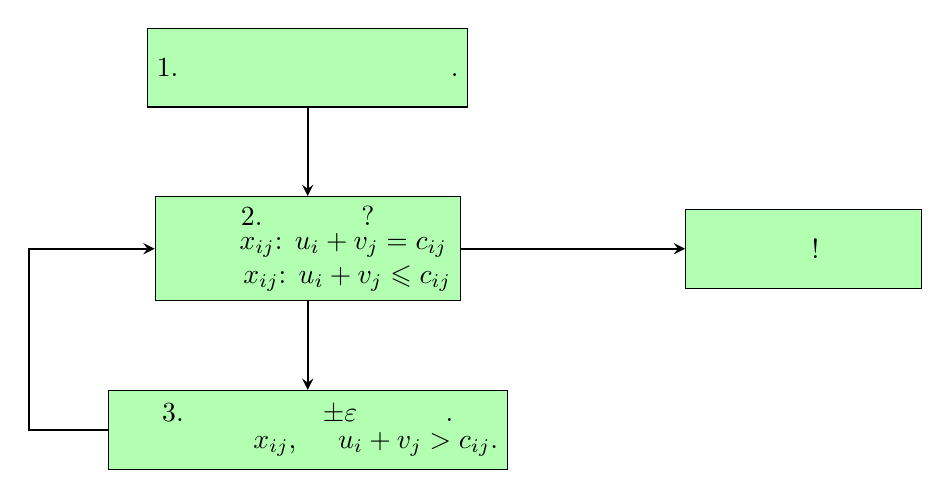
\begin{tikzpicture}[node distance=2.3cm]

  \node (start) [normal] {1. Берём базисное допустимое решение.};
  \node (quest) [decision, below of=start] {\shortstack{2. Это оптимум? \\Базисная $x_{ij}$: $u_i + v_j = c_{ij}$ \\ Свободная $x_{ij}$: $u_i + v_j \leq c_{ij}$}};
  
  \node (end) [normal, right of=quest, xshift=4cm] {Ура!};
  \node (update) [normal, below of=quest] {\shortstack{3. Корректируем на $\pm \varepsilon$  по цепочке. \\ Начинаем с любой $x_{ij}$, где $u_i + v_j > c_{ij}$. }};
  
  \draw [arrow] (start) -- (quest);
  \draw [arrow] (quest) -- node[anchor=west] {нет} (update);
  \draw [arrow] (quest) -- node[anchor=south] {да}  (end);
  \draw [arrow] (update.west)  -|  ++(-1,0)  |-  (quest.west);
  
\end{tikzpicture}
  


\begin{problem}
  Рассмотрим сбалансированную транспортную задачу
  \[
  \begin{cases}
    \sum_{ij} c_{ij} x_{ij} \to \min \\
    \sum_j x_{ij} = a_i \text{ для любого } i \\
    \sum_i x_{ij} = b_j \text{ для любого } j \\
    \text{все } x_{ij} \geq 0. \\
  \end{cases}  
  \]

  \begin{enumerate}
    \item Может ли измениться оптимальная точка, если каждый элемент матрицы $C$ увеличить в 2 раза?
    \item Может ли измениться оптимальная точка, если один столбец матрицы $C$ увеличить в 2 раза?
    \item Может ли измениться оптимальная точка, если одну строку матрицы $C$ увеличить в 2 раза?
    \item Может ли измениться оптимальная точка, если к каждому элементу матрицы $C$ прибавить 1?
    \item Может ли измениться оптимальная точка, если в одном столбце матрицы $C$ к каждому элементу прибавить 1?
    \item Может ли измениться оптимальная точка, если в одной строке матрицы $C$ к каждому элементу прибавить 1?
  \end{enumerate}

  \begin{sol}
  
  \end{sol}
\end{problem}



\begin{problem}
  Рассмотрим сбалансированную транспортную задачу
  \[
  \begin{cases}
    8x_{11} + 5x_{12} + 4x_{13} + 6x_{21} + 7 x_{22} + 3x_{23} \to \min \\
    x_{11} + x_{12} + x_{13} = 10 \\
    x_{21} + x_{22} + x_{23} = 20 \\
    x_{11} + x_{21} = 7 \\
    x_{12} + x_{22} = 11 \\
    x_{13} + x_{23} = 12 \\
    \text{все } x_{ij} \geq 0. \\
  \end{cases}  
  \]
  \begin{enumerate}
    \item Запишите задачу в виде симплекс-таблицы.
    \item Какая линейная зависимость существует между уравнениями?
    \item Сколько должно быть базисных и сколько свободных переменных?
    \item Запишите задачу в виде транспортной таблицы. 
    \item Найдите базисное допустимое решение методом северо-западного угла. 
    \item Найдите базисное допустимое решение методом минимального элемента. 
    \item Запишите двойственную задачу. 
    \item Запишите условия дополняющей нежёсткости.
    \item Найдите хотя бы одно оптимальное решение. 
  \end{enumerate}

  \begin{sol}
    \begin{enumerate}
      \item 
      \item $\text{Eq}_1 + \text{Eq}_2 = \text{Eq}_3 + \text{Eq}_4 + \text{Eq}_5$;
      \item 4 базисных переменных и 2 свободных;
      \item 
      \item 
      \[
        X = \begin{pmatrix}
           & & 0 \\
         0 &  & \\
        \end{pmatrix}  
        \]  
      \item 
      \[
        X = \begin{pmatrix}
           & & \\
          &  & \\
        \end{pmatrix}  
        \]  
      \item 
      \item 
      \[
      X = \begin{pmatrix}
         & & \\
        &  & \\
      \end{pmatrix}  
      \]
    \end{enumerate}
    
  \end{sol}
\end{problem}


\begin{problem}
  Рассмотрим сбалансированную транспортную задачу
  \[
  \begin{cases}
    10x_{11} + 8x_{12} + 9x_{13} + 5x_{21} + 2 x_{22} + 3x_{23}  + \\
    +6x_{31} + 7x_{32} + 4x_{33} + 7x_{41} + 6 x_{42} + 8x_{43} \to \min \\
    \sum_i x_{i1} = 25, \sum_i x_{i2} = 25, \sum_i x_{i3} = 50, \\  
    \sum_j x_{1j} = 15, \sum_j x_{2j} = 20, \sum_j x_{3j} = 30, \sum_j x_{4j} = 35, \\
    \text{все } x_{ij} \geq 0. \\
  \end{cases}  
  \]
  \begin{enumerate}
    \item Запишите задачу в виде транспортной таблицы. 
    \item Запишите двойственную задачу. 
    \item Найдите базисное допустимое решение методом северо-западного угла. 
    \item Найдите базисное допустимое решение методом минимального элемента. 
    \item Найдите хотя бы одно оптимальное решение. 
  \end{enumerate}

  \begin{sol}
  
  \end{sol}
\end{problem}







\begin{problem}
  Рассмотрим сбалансированную транспортную задачу, в которой 3 производителя и 7 потребителей. 
  \begin{enumerate}
    \item Сколько всего переменных в этой задаче?
    \item Сколько базисных и сколько свободных переменных в этой задаче?
    \item Сколько переменных в двойственной задаче?
    \item Сколько уравнений в условиях дополняющей нежёсткости?
  \end{enumerate}

  \begin{sol}
  \begin{enumerate}
    \item $3 \cdot 7 = 21$;
    \item $3 + 7 - 1 = 9$, $21 - 9 = 12$;
    \item $3 + 7 = 10$;
    \item $10 + 21 = 31$;
  \end{enumerate}
  \end{sol}
\end{problem}


\begin{problem}
В каждой транспортной таблице выписано базисное допустимое решение. 
Определите, какие переменные должны быть базисными, какие должны быть свободными,
а какие могут быть базисными или свободными.
  \begin{enumerate}
    \item 
    \begin{tabular}{c|c|c|c|}
      &  &  &  \\ \hline
     & 5 & $x_{12}$ & $x_{13}$ \\ \hline
    & $x_{21}$ & 7 & 8 \\ \hline
     & $x_{31}$ & $x_{32}$ & 3 \\ \hline
    \end{tabular}

    \item 
    \begin{tabular}{c|c|c|c|}
      &  &  &  \\ \hline
     & 5 & $x_{12}$ & $x_{13}$ \\ \hline
    & 3 & $x_{22}$ & 8 \\ \hline
     & $x_{31}$ & $x_{32}$ & 3 \\ \hline
    \end{tabular}

    \item 
    \begin{tabular}{c|c|c|c|}
      &  &  &  \\ \hline
     & 5 & $x_{12}$ & $x_{13}$ \\ \hline
    & 3 & $x_{22}$ & $x_{23}$ \\ \hline
     & $9$ & $x_{32}$ & 3 \\ \hline
    \end{tabular}

    \item 
    \begin{tabular}{c|c|c|c|c|c|}
      &  &  &  & & \\ \hline
      & 5 & $x_{12}$ & 4 & $x_{34}$ & 7 \\ \hline
      & 2 & $x_{22}$ & $x_{23}$ & 3 & $x_{25}$ \\ \hline
     & $x_{31}$ & $x_{32}$ & 2 & $x_{34}$ & $x_{35}$ \\ \hline
     & $x_{41}$ & 7 & $x_{43}$ & $x_{44}$ & $x_{45}$ \\ \hline
    \end{tabular}
  \end{enumerate}
  \begin{sol}
    Буквой «Б» отмечены переменные, которые обязательно являются базисными. 
    Буквой «С» отмечены переменные, которые обязательно являются свободными.
    Надписью «Б или С» отмечены переменные, которые могут быть базисными или свободными.

    \begin{enumerate}
      \item 
      \begin{tabular}{c|c|c|c|}
        &  &  &  \\ \hline
       & Б & Б или С & Б или С \\ \hline
      & Б или С & Б & Б \\ \hline
       & Б или С & С & Б \\ \hline
      \end{tabular}
  
      \item 
      \begin{tabular}{c|c|c|c|}
        &  &  &  \\ \hline
        & Б & Б или С & С \\ \hline
        & Б & Б или С & Б \\ \hline
         & С & Б или С & Б \\ \hline
        \end{tabular}
  
      \item 
      \begin{tabular}{c|c|c|c|}
        &  &  &  \\ \hline
        & Б & Б или С & C \\ \hline
        & Б & Б или С & C \\ \hline
         & Б & Б или С & Б \\ \hline
        \end{tabular}
  
      \item 
      \begin{tabular}{c|c|c|c|c|c|}
        &  &  &  & & \\ \hline
        & Б & Б или С & Б & C & Б \\ \hline
        & Б & Б или С & C & Б & C \\ \hline
        & C & Б или С & Б & C & C \\ \hline
        & Б или С & Б & Б или С & Б или С & Б или С \\ \hline  
      \end{tabular}
    \end{enumerate}
  
    
  \end{sol}
\end{problem}


\begin{problem}
  
  \begin{sol}
\begin{tabular}{c|C|C|C|}
      & $b_1 = 10$         & $b_2 = 20$             & $b_3 = 17$         \\\hline
$a_1 = 5$ & \innerbox{}{12}   & \innerbox{}{10}   & \innerbox{600}{6}   \\\hline
$a_2 = 6$ & \innerbox{400}{4} & \innerbox{}{15}   & \innerbox{}{3}       \\\hline
$a_3 = 7$ & \innerbox{300}{9} & \innerbox{}{7}    & \innerbox{}{M}       \\\hline
$a_4 = 5$ & \innerbox{}{11}   & \innerbox{500}{8} & \innerbox{300}{6}   \\\hline
\end{tabular}

  \end{sol}
\end{problem}

\section{Сети}









\subsection*{Алгоритм Дейкстры, Dijkstra algorithm}

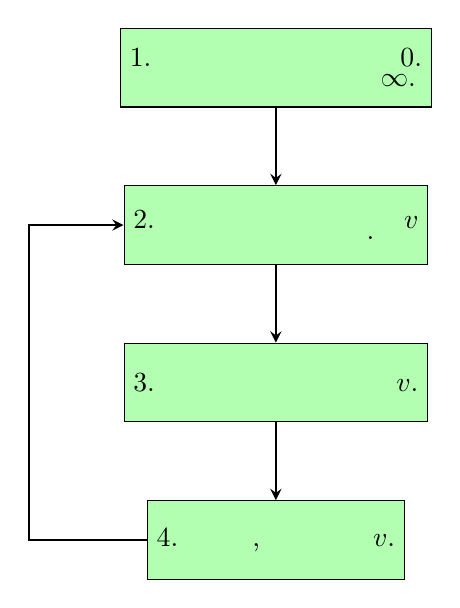
\begin{tikzpicture}[node distance=2cm]

  \node (start) [normal] {\shortstack{1. Стартовой вершине присваиваем $0$.\\
  Остальным вершинам присваиваем $\infty$.}};
  \node (select) [normal, below of=start] {\shortstack{2. Выбираем непосещённую вершину $v$ \\ с минимальной стоимостью. }};
  \node (update) [normal, below of=select] {\shortstack{3. Исправляем стоимости соседей $v$. }};
  \node (mark) [normal, below of=update] {\shortstack{4. Отмечаем, что посетили $v$. }};

  \draw [arrow] (start) -- (select);
  \draw [arrow] (select) --  (update);
  \draw [arrow] (update) -- (mark);
  \draw [arrow] (mark.west)  -| ++(-1.5,0)  |-  (select.west);
  
\end{tikzpicture}
  

\begin{problem}

  На ребрах графа указано время в пути.
  
  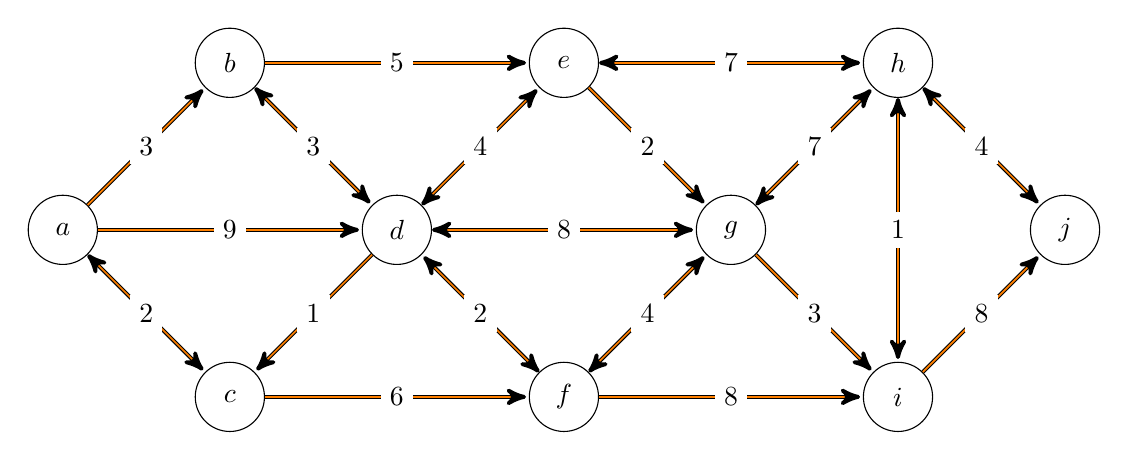
\begin{tikzpicture}[>=stealth',shorten >=1pt,node distance=3cm,on grid,initial/.style    ={}]
    \node[state]     (A)                        {$a$};
    \node[state]     (B) [above right =of A]    {$b$};
    \node[state]     (C) [below right =of A]    {$c$};
    \node[state]     (D) [below right =of B]    {$d$};
    \node[state]     (E) [above right =of D]    {$e$};
    \node[state]     (F) [below right =of D]    {$f$};
    \node[state]     (G) [above right =of F]    {$g$};
    \node[state]     (H) [above right =of G]    {$h$};
    \node[state]     (I) [below right =of G]    {$i$};
    \node[state]     (J) [above right =of I]    {$j$};
  
  
  \tikzset{mystyle/.style={->,double=orange}} 
  \tikzset{every node/.style={fill=white}} 
  \path (A)     edge [mystyle]    node   {$3$} (B)
        (B)     edge [mystyle]    node   {$5$} (E)
        (C)     edge [mystyle]    node   {$6$} (F)
        (G)     edge [mystyle]    node   {$3$} (I)
        (E)     edge [mystyle]    node   {$2$} (G)
        (F)     edge [mystyle]    node   {$8$} (I)
        (D)     edge [mystyle]    node   {$1$} (C)
        (I)     edge [mystyle]    node   {$8$} (J)
        (A)     edge [mystyle]    node   {$9$} (D);
  \tikzset{mystyle/.style={<->,double=orange}}   
  \path (A)     edge [mystyle]   node   {$2$} (C)
        (B)     edge [mystyle]    node   {$3$} (D)
        (D)     edge [mystyle]   node   {$4$} (E)
        (G)     edge [mystyle]    node   {$7$} (H)
        (F)     edge [mystyle]    node   {$2$} (D)
        (H)     edge [mystyle]    node   {$4$} (J)
        (D)     edge [mystyle]    node   {$8$} (G)
        (E)     edge [mystyle]    node   {$7$} (H)
        (H)     edge [mystyle]    node   {$1$} (I)
        (F)     edge [mystyle]   node   {$4$} (G);
  % \tikzset{mystyle/.style={<->,relative=false,in=0,out=60,double=orange}}
  % \path (F)     edge [mystyle]   node   {$10$} (E); 
  \end{tikzpicture}
  
  \begin{enumerate}
    \item С помощью алгоритма Дейкстры найдите самые быстрые маршруты из вершины $a$ во все остальные вершины.
    \item Выпишите матрицу весов для куска графа из вершин $a$, $b$, $c$ и $d$.
  \end{enumerate}
  
  
  \begin{sol}
  \end{sol}
  \end{problem}
  


\begin{problem}

  С помощью алгоритма Дейкстры найдите кратчайшее расстояние из точки старта $s$ до каждой точки лабиринта. 

  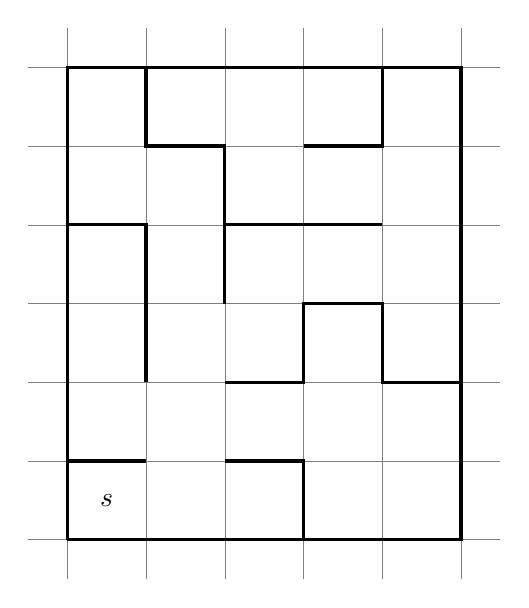
\begin{tikzpicture}
    \draw[help lines] (0.5,0.5) grid (6.5,7.5);
    \draw[] (1.5,1.5) node(s){$s$};
    \draw[very thick] (1,1)--(1,2)--(2,2);
    \draw[very thick] (4,6)--(5,6)--(5,7);
    \draw[very thick] (3,2)--(4,2)--(4,1)--(5,1);
    \draw[very thick] (1,4)--(1,5)--(2,5)--(2,4)--(2,3);
    \draw[very thick] (2,7)--(2,6)--(3,6)--(3,5)--(3,4);
    \draw[very thick] (3,3)--(4,3)--(4,4)--(5,4)--(5,3)--(6,3);
    \draw[very thick] (3,5)--(4,5)--(5,5);
    \draw[very thick] (3,2)--(4,2);
    \draw[very thick] (1,1)--(6,1)--(6,7)--(1,7)--(1,1);
  \end{tikzpicture}
    
  \begin{sol}
  \end{sol}
\end{problem}

\begin{problem}
Матрица весов взвешенного графа равна
\[
  M = \begin{pmatrix}
    \infty & 4 & \infty & 2 \\
    2 & \infty & 1 & \infty \\
    3 & 4 & \infty & 1 \\
    5 & 6 & \infty & \infty \\
  \end{pmatrix}.
\]

Нарисуйте граф. 

\begin{sol}
\end{sol}
\end{problem}


\begin{problem}
  Матрица смежности графа равна
  \[
    M = \begin{pmatrix}
      0 & 0 & 1 & 1 \\
      0 & 0 & 1 & 0 \\
      1 & 1 & 0 & 1 \\
      1 & 0 & 1 & 0 \\
    \end{pmatrix}.
  \]
  
  \begin{enumerate}
    \item  Нарисуйте граф. 
    \item Найдите матрицу $A = M^2$. Какой смысл у элемента $a_{44}$? Какой смысл у элемента $a_{31}$?
    \item Найдите матрицу $B = M^3$. Какой смысл у элемента $b_{31}$? Какой смысл у элемента $b_{32}$?
  \end{enumerate}


\begin{sol}
\end{sol}
\end{problem}

\subsection*{Задача о максимальном потоке и о минимальном разрезе}

\begin{leftbar}
  \begin{itemize}
  \item пропускная способность, capacity, \chinesetext{大流量?};
  \item поток, flow, \chinesetext{流};
  \item источник, source, \chinesetext{源};
  \item сток, sink, \chinesetext{汇};
  \item разрез, cut, \chinesetext{割};
  \item бутылочное горлышко, bottleneck, \chinesetext{瓶颈};
  \item минимальный разрез, minimal cut, \chinesetext{最小割};
  \item увеличивающая цепь, augmenting path, \chinesetext{增广路径}, zēng guǎng lu jing;
  \item остаточная пропускная способность, residual capacity, \chinesetext{残留容量};
  \end{itemize}
\end{leftbar}

Хорошие слайды можно найти у Кляйнберга и Тардос, \cite{kleinberg2014algo}.

алгоритм Форда~— Фалкерсона, Ford~— Fulkerson algorithm, \chinesetext{?};

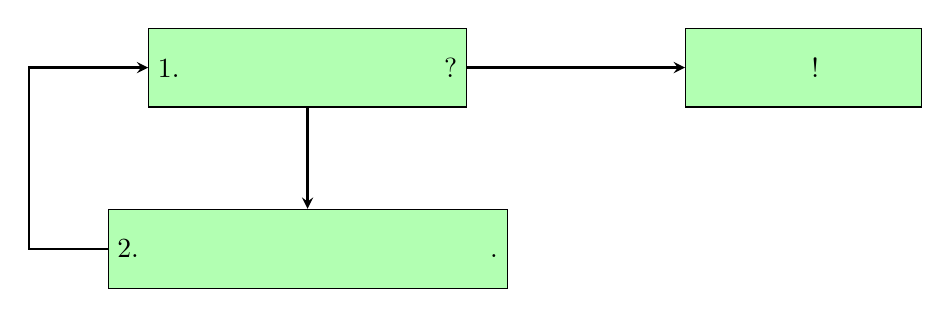
\begin{tikzpicture}[node distance=2.3cm]
  
  \node (quest) [decision] {1. Существует ли увеличивающая цепь?};
  
  \node (end) [normal, right of=quest, xshift=4cm] {Ура!};
  \node (update) [normal, below of=quest] {2. Корректируем поток вдоль увеличивающей цепи.};
  

  \draw [arrow] (quest) -- node[anchor=west] {да} (update);
  \draw [arrow] (quest) -- node[anchor=south] {нет}  (end);
  \draw [arrow] (update.west)  -|  ++(-1,0)  |-  (quest.west);
  
\end{tikzpicture}
  

\begin{problem}

    На ребрах графа указаны текущий поток $f$ и пропускная способность $c$.
    Например, надпись $1/3$ над ребром означает, 
    что по ребру течёт поток величины $1$, а пропускная способность ребра равна $3$.
  
    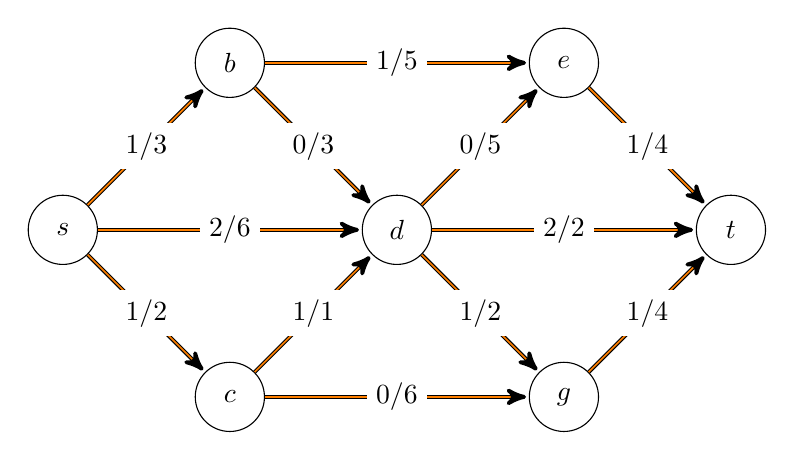
\begin{tikzpicture}[>=stealth',shorten >=1pt,node distance=3cm,on grid,initial/.style    ={}]
      \node[state]     (s)                        {$s$};
      \node[state]     (b) [above right =of s]    {$b$};
      \node[state]     (c) [below right =of s]    {$c$};
      \node[state]     (d) [below right =of b]    {$d$};
      \node[state]     (e) [above right =of d]    {$e$};
      \node[state]     (g) [below right =of d]    {$g$};
      \node[state]     (t) [above right =of g]    {$t$};
    
    
    \tikzset{mystyle/.style={->,double=orange}} 
    \tikzset{every node/.style={fill=white}} 
    \path (s)     edge [mystyle]    node   {$1/3$} (b)
    (s)     edge [mystyle]    node   {$2/6$} (d)
    (s)     edge [mystyle]    node   {$1/2$} (c)
    (b)     edge [mystyle]    node   {$0/3$} (d)
    (d)     edge [mystyle]    node   {$0/5$} (e)
    (d)     edge [mystyle]    node   {$2/2$} (t)
    (d)     edge [mystyle]    node   {$1/2$} (g)
    (g)     edge [mystyle]    node   {$1/4$} (t)
    (b)     edge [mystyle]    node   {$1/5$} (e)
    (c)     edge [mystyle]    node   {$0/6$} (g)
    (e)     edge [mystyle]    node   {$1/4$} (t)
    (c)     edge [mystyle]    node   {$1/1$} (d);
\end{tikzpicture}
    
\begin{enumerate}
\item Найдите пропускную способность разреза $c(S, T)$ для $S = \{s, b, c\}$, $T = \{e, g, t, d\}$. 
\item Найдите пропускную способность разреза $c(S, T)$ для $S = \{s, g, e\}$, $T = \{b, c, t, d\}$. 
\item Найдите величину потока $v(f)$.
\item Найдите исходящий поток $f^{\text{out}}(S)$ и входящий поток $f^{\text{in}}(S)$ для множества $S = \{s, b, g, e\}$.
\item Найдите остаточную пропускную способность $\bneck(s- b- e- t, f)$.
\item Найдите остаточную пропускную способность $\bneck(s- c- g- d- e- t, f)$.      
\end{enumerate}

\begin{sol}

  \begin{enumerate}
    \item $c(S, T) = 5 + 3 + 6 + 1 + 6 = 21$;
    \item $c(S, T) = 3 + 6 + 4 + 4 + 2 = 19$;
    \item $v(f) = 4$;
    \item $f^{\text{out}}(S) = 0 + 2+ 1+ 1 + 1 = 5$, $f^{\text{in}}(S) = 1 + 0 + 0 = 1$;
    \item $\bneck(s- b- e- t, f) = \min\{2, 4, 3\} = 2$;
    \item $\bneck(s- c- g- d- e- t, f) = \min \{1, 6, 1, 5, 3\} = 1$.      
  \end{enumerate}
    
\end{sol}
\end{problem}


    \begin{problem}

      Надпись $f/c$ на ребре означает текущий поток $f$ и пропускную способность $c$.
    
      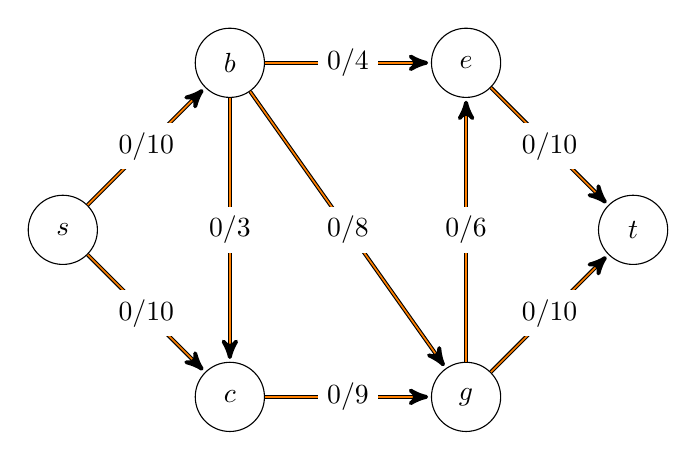
\begin{tikzpicture}[>=stealth',shorten >=1pt,node distance=3cm,on grid,initial/.style    ={}]
        \node[state]     (s)                        {$s$};
        \node[state]     (b) [above right =of s]    {$b$};
        \node[state]     (c) [below right =of s]    {$c$};
        \node[state]     (e) [right =of b]    {$e$};
        \node[state]     (g) [right =of c]    {$g$};
        \node[state]     (t) [above right =of g]    {$t$};
      
      
      \tikzset{mystyle/.style={->,double=orange}} 
      \tikzset{every node/.style={fill=white}} 
      \path (s)     edge [mystyle]    node   {$0/10$} (b)
      (s)     edge [mystyle]    node   {$0/10$} (c)
      (b)     edge [mystyle]    node   {$0/8$} (g)
      (g)     edge [mystyle]    node   {$0/10$} (t)
      (b)     edge [mystyle]    node   {$0/4$} (e)
      (g)     edge [mystyle]    node   {$0/6$} (e)
      (c)     edge [mystyle]    node   {$0/9$} (g)
      (e)     edge [mystyle]    node   {$0/10$} (t)
      (b)     edge [mystyle]    node   {$0/3$} (c);
  \end{tikzpicture}

  \begin{enumerate}
    \item С помощью алгоритма Форда~— Фалкерсона найдите максимальный поток.
    \item Укажите минимальный разрез. 
    \item Запишите задачу максимизации потока как задачу линейного программирования.
  \end{enumerate}
  

\begin{sol}
  \begin{enumerate}
    \item $\max v(f) = 19$;
    
    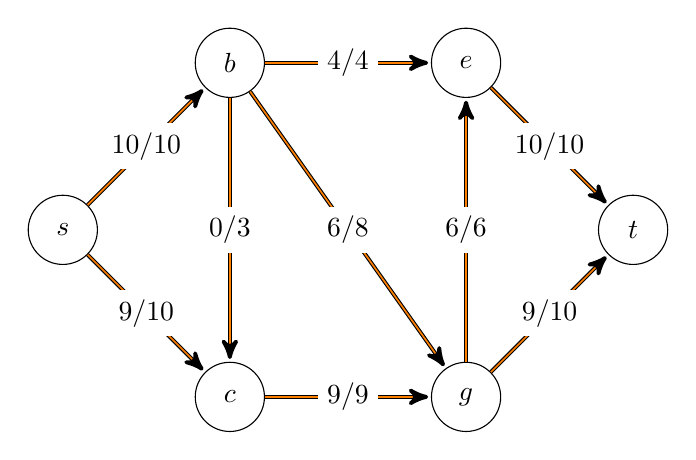
\begin{tikzpicture}[>=stealth',shorten >=1pt,node distance=3cm,on grid,initial/.style    ={}]
      \node[state]     (s)                        {$s$};
      \node[state]     (b) [above right =of s]    {$b$};
      \node[state]     (c) [below right =of s]    {$c$};
      \node[state]     (e) [right =of b]    {$e$};
      \node[state]     (g) [right =of c]    {$g$};
      \node[state]     (t) [above right =of g]    {$t$};
    
    
    \tikzset{mystyle/.style={->,double=orange}} 
    \tikzset{every node/.style={fill=white}} 
    \path (s)     edge [mystyle]    node   {$10/10$} (b)
    (s)     edge [mystyle]    node   {$9/10$} (c)
    (b)     edge [mystyle]    node   {$6/8$} (g)
    (g)     edge [mystyle]    node   {$9/10$} (t)
    (b)     edge [mystyle]    node   {$4/4$} (e)
    (g)     edge [mystyle]    node   {$6/6$} (e)
    (c)     edge [mystyle]    node   {$9/9$} (g)
    (e)     edge [mystyle]    node   {$10/10$} (t)
    (b)     edge [mystyle]    node   {$0/3$} (c);
\end{tikzpicture}  
    \item $\min c(S, T) = 19$, $S = \{ s, c\}$, $T = \{ b, g, e, t\}$.
  \end{enumerate}
\end{sol}
\end{problem}








\begin{problem}

      На ребрах графа с помощью $f/c$ указаны текущий поток $f$ и пропускная способность $c$.
    
      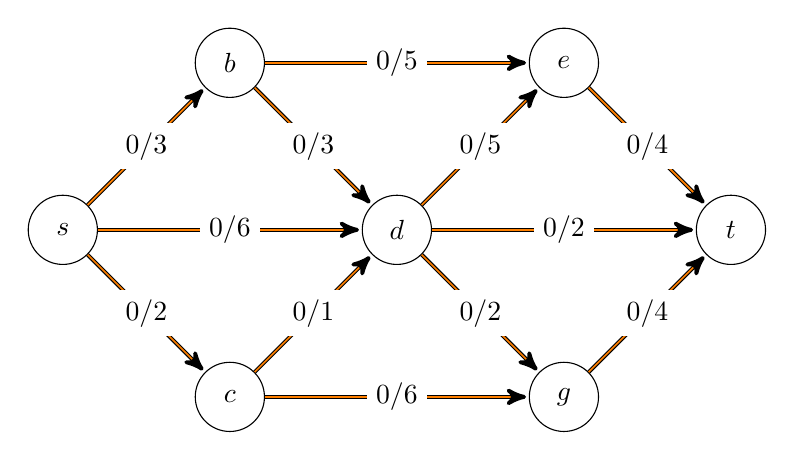
\begin{tikzpicture}[>=stealth',shorten >=1pt,node distance=3cm,on grid,initial/.style    ={}]
        \node[state]     (s)                        {$s$};
        \node[state]     (b) [above right =of s]    {$b$};
        \node[state]     (c) [below right =of s]    {$c$};
        \node[state]     (d) [below right =of b]    {$d$};
        \node[state]     (e) [above right =of d]    {$e$};
        \node[state]     (g) [below right =of d]    {$g$};
        \node[state]     (t) [above right =of g]    {$t$};
      
      
      \tikzset{mystyle/.style={->,double=orange}} 
      \tikzset{every node/.style={fill=white}} 
      \path (s)     edge [mystyle]    node   {$0/3$} (b)
      (s)     edge [mystyle]    node   {$0/6$} (d)
      (s)     edge [mystyle]    node   {$0/2$} (c)
      (b)     edge [mystyle]    node   {$0/3$} (d)
      (d)     edge [mystyle]    node   {$0/5$} (e)
      (d)     edge [mystyle]    node   {$0/2$} (t)
      (d)     edge [mystyle]    node   {$0/2$} (g)
      (g)     edge [mystyle]    node   {$0/4$} (t)
      (b)     edge [mystyle]    node   {$0/5$} (e)
      (c)     edge [mystyle]    node   {$0/6$} (g)
      (e)     edge [mystyle]    node   {$0/4$} (t)
      (c)     edge [mystyle]    node   {$0/1$} (d);
  \end{tikzpicture}

  \begin{enumerate}
    \item С помощью алгоритма Форда~— Фалкерсона найдите максимальный поток.
    \item Укажите минимальный разрез. 
    \item Запишите задачу максимизации потока как задачу линейного программирования.
  \end{enumerate}
  

\begin{sol}
\begin{enumerate}
\item $\max v(f) = 10$;

Один из возможных вариантов:

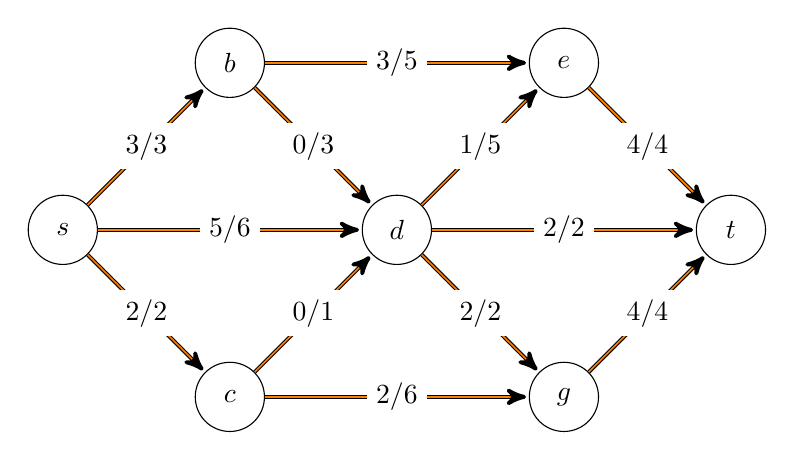
\begin{tikzpicture}[>=stealth',shorten >=1pt,node distance=3cm,on grid,initial/.style    ={}]
  \node[state]     (s)                        {$s$};
  \node[state]     (b) [above right =of s]    {$b$};
  \node[state]     (c) [below right =of s]    {$c$};
  \node[state]     (d) [below right =of b]    {$d$};
  \node[state]     (e) [above right =of d]    {$e$};
  \node[state]     (g) [below right =of d]    {$g$};
  \node[state]     (t) [above right =of g]    {$t$};


\tikzset{mystyle/.style={->,double=orange}} 
\tikzset{every node/.style={fill=white}} 
\path (s)     edge [mystyle]    node   {$3/3$} (b)
(s)     edge [mystyle]    node   {$5/6$} (d)
(s)     edge [mystyle]    node   {$2/2$} (c)
(b)     edge [mystyle]    node   {$0/3$} (d)
(d)     edge [mystyle]    node   {$1/5$} (e)
(d)     edge [mystyle]    node   {$2/2$} (t)
(d)     edge [mystyle]    node   {$2/2$} (g)
(g)     edge [mystyle]    node   {$4/4$} (t)
(b)     edge [mystyle]    node   {$3/5$} (e)
(c)     edge [mystyle]    node   {$2/6$} (g)
(e)     edge [mystyle]    node   {$4/4$} (t)
(c)     edge [mystyle]    node   {$0/1$} (d);
\end{tikzpicture}

\item $\min c(S, T) = 10$,  $S = \{s, b, c, d, e, g\}$, $T = \{ t\}$.
\item 
\[
\begin{cases}
  x_{sb} + x_{sc} + x_{sd} \to \max \\
  \text{все } x_{ij} \geq 0 \\
  x_{sb} \leq 3, x_{sd} \leq 6, x_{sc} \leq 2, x_{bd} \leq 3, x_{be} \leq 5 \\
  x_{cg} \leq 6, x_{cd} \leq 1, x_{de} \leq 5, x_{dt} \leq 2, x_{dg} \leq 2 \\
  x_{et} \leq 4, x_{gt} \leq 4 \\
  x_{sb} = x_{bd} + x_{be}, x_{be} + x_{de} = x_{et}, x_{sc} = x_{cd} + x_{cg} \\
  x_{dg} + x_{cg} = x_{gt}, x_{sd} + x_{bd} + x_{cd} = x_{de} + x_{dt} + x_{dg}
\end{cases}
\]
\end{enumerate}

\end{sol}
\end{problem}


\begin{problem}

Надпись $f/c$ на ребре означает текущий поток $f$ и пропускную способность $c$.

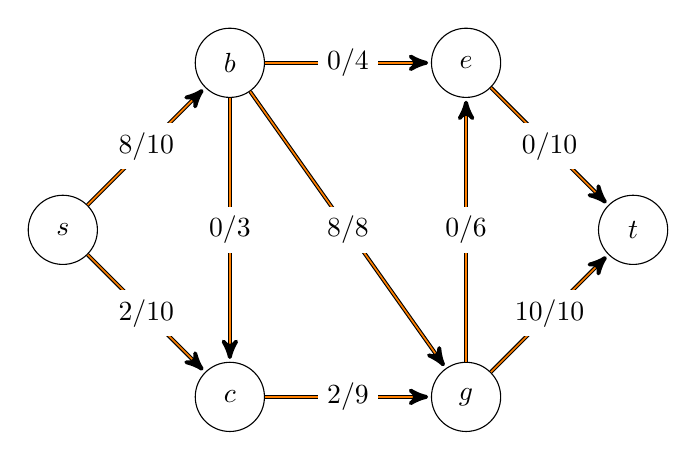
\begin{tikzpicture}[>=stealth',shorten >=1pt,node distance=3cm,on grid,initial/.style    ={}]
\node[state]     (s)                        {$s$};
\node[state]     (b) [above right =of s]    {$b$};
\node[state]     (c) [below right =of s]    {$c$};
\node[state]     (e) [right =of b]    {$e$};
\node[state]     (g) [right =of c]    {$g$};
\node[state]     (t) [above right =of g]    {$t$};


\tikzset{mystyle/.style={->,double=orange}} 
\tikzset{every node/.style={fill=white}} 
\path (s)     edge [mystyle]    node   {$8/10$} (b)
(s)     edge [mystyle]    node   {$2/10$} (c)
(b)     edge [mystyle]    node   {$8/8$} (g)
(g)     edge [mystyle]    node   {$10/10$} (t)
(b)     edge [mystyle]    node   {$0/4$} (e)
(g)     edge [mystyle]    node   {$0/6$} (e)
(c)     edge [mystyle]    node   {$2/9$} (g)
(e)     edge [mystyle]    node   {$0/10$} (t)
(b)     edge [mystyle]    node   {$0/3$} (c);
\end{tikzpicture}

\begin{enumerate}
\item Найдите пропускную способность разреза $c(S, T)$ для $S = \{s, b, c\}$ и $T = \{e, g, t\}$.
\item Найдите пропускную способность разреза $c(S, T)$ для $S = \{s, g, e\}$ и $T = \{b, c, t\}$.
\item Найдите величину потока $v(f)$.
\item Найдите исходящий поток $f^{\text{out}}(S)$ и входящий поток $f^{\text{in}}(S)$ для множества $S = \{s, c, g\}$.
\item Найдите остаточную пропускную способность $\bneck(s- b- e- t, f)$.
\item Найдите остаточную пропускную способность $\bneck(s- c- g- b- e - t, f)$.      
\end{enumerate}


\begin{sol}
  \begin{enumerate}
    \item $c(S, T) = 4 + 8 + 9 = 21$;
    \item $c(S, T) = 10 + 10 + 10 + 10 = 40$; 
    \item $v(f) = 2 + 8 = 10$.
    \item $f^{\text{out}}(S)$ и входящий поток $f^{\text{in}}(S)$ для множества $S = \{s, c, g\}$.
    \item $\bneck(s- b- e- t, f) = \min\{2, 4, 10 \} = 2$.
    \item $\bneck(s- c- g- b- e - t, f) = \min\{8, 7, 8, 4, 10 \} = 4$.      
    \end{enumerate}
    
\end{sol}
\end{problem}

\subsection*{Меры центральности}

\begin{leftbar}
 \begin{itemize}
  \item Степень вершины, degree of the vertex, $\deg(v)$.
  \item Центральность по близости, closeness centrality,
  \[
    \closeness(v) = \frac{1}{\sum_x d(v, x)},
  \]
  где $d(v, x)$ — кратчайшее расстояние между вершинами $v$ и $x$.
  \item Центральность по количеству кратчайших путей, betweenness centrality,
  \[
    \betweenness(v) = \sum_{v \neq a, v \neq b, \\ a \neq b} \frac{N_v(a, b)}{N(a, b)},
  \]
  где $N(a, b)$ — количество кратчайших путей между вершинами $a$ и $b$,
  $N_v(a, b)$ — количество кратчайших путей между вершинами $a$ и $b$, проходящих через вершину $v$.
 \end{itemize}

\end{leftbar}

\begin{problem}

Рассмотрим следующий граф:

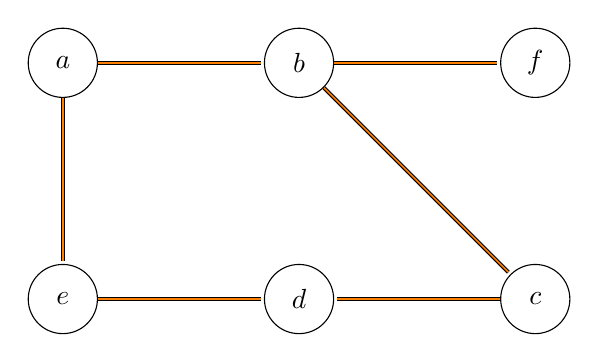
\begin{tikzpicture}[>=stealth',shorten >=1pt,node distance=3cm,on grid,initial/.style    ={}]
\node[state]     (a)                        {$a$};
\node[state]     (b) [right =of a]    {$b$};
\node[state]     (e) [below =of a]    {$e$};
\node[state]     (d) [right =of e]    {$d$};
\node[state]     (f) [right =of b]    {$f$};
\node[state]     (c) [right =of d]    {$c$};

\tikzset{mystyle/.style={-,double=orange}}
\tikzset{every node/.style={fill=white}}
\path (a)     edge [mystyle]    (b)
(a)     edge [mystyle]     (e)
(b)     edge [mystyle]     (c)
(e)     edge [mystyle]     (d)
(c)     edge [mystyle]     (d)
(b)     edge [mystyle]     (f);
\end{tikzpicture}


\begin{enumerate}
 \item Найдите степень каждой вершины, $\deg(v)$.
 \item Найдите центральность каждой вершины по близости, $\closeness(v)$.
 \item Найдите центральность каждой вершины по числу кратчайших путей, $\betweenness(v)$.
\end{enumerate}

\begin{sol}

\end{sol}
\end{problem}


\begin{problem}

Рассмотрим следующий граф:

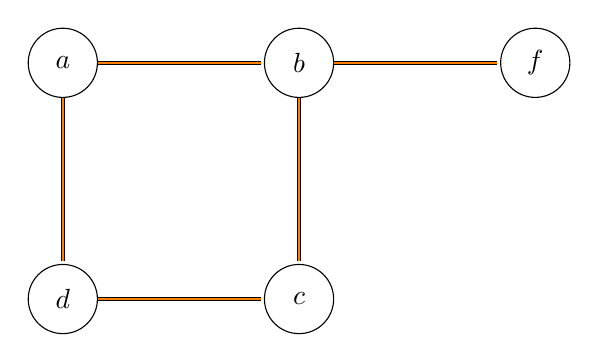
\begin{tikzpicture}[>=stealth',shorten >=1pt,node distance=3cm,on grid,initial/.style    ={}]
\node[state]     (a)                        {$a$};
\node[state]     (b) [right =of a]    {$b$};
\node[state]     (d) [below =of a]    {$d$};
\node[state]     (c) [right =of d]    {$c$};
\node[state]     (f) [right =of b]    {$f$};

\tikzset{mystyle/.style={-,double=orange}}
\tikzset{every node/.style={fill=white}}
\path (a)     edge [mystyle]    (b)
(a)     edge [mystyle]     (d)
(b)     edge [mystyle]     (c)
(d)     edge [mystyle]     (c)
(b)     edge [mystyle]     (f);
\end{tikzpicture}


\begin{enumerate}
 \item Найдите степень каждой вершины, $\deg(v)$.
 \item Найдите центральность каждой вершины по близости, $\closeness(v)$.
 \item Найдите центральность каждой вершины по числу кратчайших путей, $\betweenness(v)$.
\end{enumerate}

\begin{sol}

\end{sol}
\end{problem}



\section{Неравенства}


\begin{leftbar}
\begin{itemize}
 \item AM/GM inequality,
 \[
   (x_1 + x_2 + \ldots + x_n) / n \geq  \sqrt[n]{x_1 x_2 \cdots x_n}.
 \]
\item Неравенство Коши~— Буняковского, Cauchy~— Schwarz inequality,
\[
   \abs{\scalp{a, b}} \leq \norm{a} \norm{b},
\]
где $\norm{a} = \sqrt{a_1^2 + \ldots + a_n^2}$, $\scalp{a, b} = a_1 b_1 + \ldots + a_n b_n$.
\end{itemize}


\end{leftbar}



\begin{problem}
Найдите условные экстремумы:
\begin{enumerate}
 \item $xyz \to \max$ при условии $x + y + z = 600$, $x \geq 0$, $y \geq 0$, $z \geq 0$.
 \item $xy \to \max$ при условии $2x + y = 600$, $x \geq 0$, $y \geq 0$.
 \item $xy \to \max$ при условии $2x + y = 400$, $x \geq 0$, $y \geq 0$.
 \item $x^2y \to \max$ при условии $x + y = 300$, $x \geq 0$, $y \geq 0$.
 \item $x^3y^5 \to \max$ при условии $6x + 7y = 200$, $x \geq 0$, $y \geq 0$.
 \item $a + b + c \to \min$ при условии $abc = 100$, $a \geq 0$, $b \geq 0$, $c \geq 0$.
 \item $a^2 + b^2 + c^2 \to \min$ при условии $abc = 100$, $a \geq 0$, $b \geq 0$, $c \geq 0$.
 \item $ab + bc + ac \to \min$ при условии $abc = 100$, $a \geq 0$, $b \geq 0$, $c \geq 0$.
 \item $2a + 3b + 4c \to \min$ при условии $abc = 100$, $a \geq 0$, $b \geq 0$, $c \geq 0$.
 \item $2ab + 3bc + 4ac \to \min$ при условии $abc = 100$, $a \geq 0$, $b \geq 0$, $c \geq 0$.
 \item $a + b + c \to \min$ при условии $a^2 b^3 c^4 = 100$, $a \geq 0$, $b \geq 0$, $c \geq 0$.
 \item $7a + 3b + 4c \to \min$ при условии $a^2 b^3 c^4 = 100$, $a \geq 0$, $b \geq 0$, $c \geq 0$.
\end{enumerate}

\begin{sol}

\end{sol}
\end{problem}


\begin{problem}


\begin{sol}

\end{sol}
\end{problem}


\begin{problem}


\begin{sol}

\end{sol}
\end{problem}


\begin{problem}


\begin{sol}

\end{sol}
\end{problem}


\begin{problem}


\begin{sol}

\end{sol}
\end{problem}



\begin{problem}


\begin{sol}

\end{sol}
\end{problem}



\section{Динамическое программирование}


\begin{leftbar}
\begin{itemize}
 \item Принцип Беллмана, Bellman principle
\item Метод обратной индукции, backward induction
\end{itemize}
\end{leftbar}


\begin{problem}

  На ребрах графа указано время в пути.

  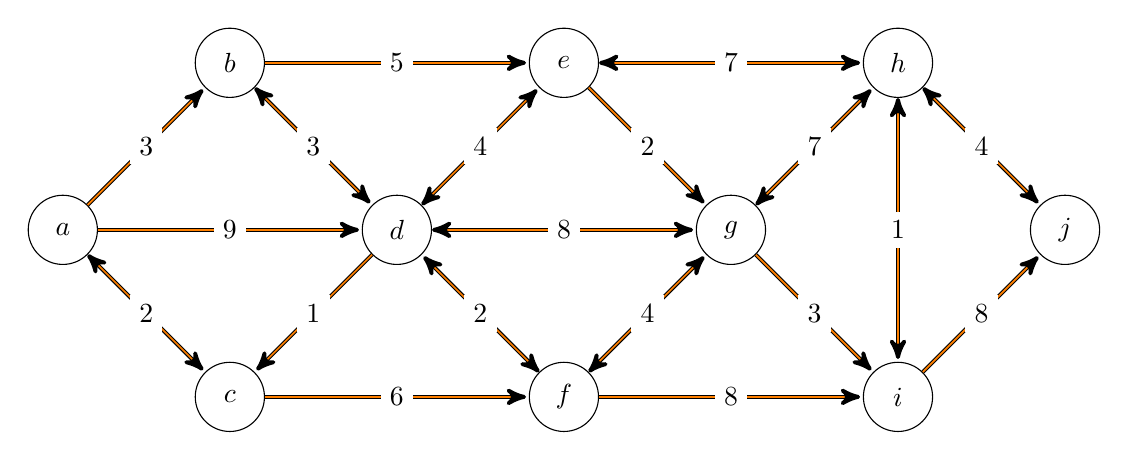
\begin{tikzpicture}[>=stealth',shorten >=1pt,node distance=3cm,on grid,initial/.style    ={}]
    \node[state]     (A)                        {$a$};
    \node[state]     (B) [above right =of A]    {$b$};
    \node[state]     (C) [below right =of A]    {$c$};
    \node[state]     (D) [below right =of B]    {$d$};
    \node[state]     (E) [above right =of D]    {$e$};
    \node[state]     (F) [below right =of D]    {$f$};
    \node[state]     (G) [above right =of F]    {$g$};
    \node[state]     (H) [above right =of G]    {$h$};
    \node[state]     (I) [below right =of G]    {$i$};
    \node[state]     (J) [above right =of I]    {$j$};


  \tikzset{mystyle/.style={->,double=orange}}
  \tikzset{every node/.style={fill=white}}
  \path (A)     edge [mystyle]    node   {$3$} (B)
        (B)     edge [mystyle]    node   {$5$} (E)
        (C)     edge [mystyle]    node   {$6$} (F)
        (G)     edge [mystyle]    node   {$3$} (I)
        (E)     edge [mystyle]    node   {$2$} (G)
        (F)     edge [mystyle]    node   {$8$} (I)
        (D)     edge [mystyle]    node   {$1$} (C)
        (I)     edge [mystyle]    node   {$8$} (J)
        (A)     edge [mystyle]    node   {$9$} (D);
  \tikzset{mystyle/.style={<->,double=orange}}
  \path (A)     edge [mystyle]   node   {$2$} (C)
        (B)     edge [mystyle]    node   {$3$} (D)
        (D)     edge [mystyle]   node   {$4$} (E)
        (G)     edge [mystyle]    node   {$7$} (H)
        (F)     edge [mystyle]    node   {$2$} (D)
        (H)     edge [mystyle]    node   {$4$} (J)
        (D)     edge [mystyle]    node   {$8$} (G)
        (E)     edge [mystyle]    node   {$7$} (H)
        (H)     edge [mystyle]    node   {$1$} (I)
        (F)     edge [mystyle]   node   {$4$} (G);
  % \tikzset{mystyle/.style={<->,relative=false,in=0,out=60,double=orange}}
  % \path (F)     edge [mystyle]   node   {$10$} (E);
  \end{tikzpicture}

  С помощью метода обратной индукции найдите самые быстрые маршруты в вершину $j$ из вершин $a$, $b$ и $c$.


  \begin{sol}
  \end{sol}
  \end{problem}


\begin{problem}
В куче лежит 2024 камня.
Бульбазавр и Пикачу берут камни из кучи по очереди.
Бульбазавр берёт камень первым.
Бульбазавр может взять 2, 3 или 5 камней за один ход.
Пикачу может взять 1 или 3 камня за один ход.

Проигрывает игру тот, кто первым не сможет сделать ход по правилам.
\begin{enumerate}
 \item Сможет ли Бульбазавр выиграть?
 \item Если Бульбазавр может выиграть, то какой первый ход ему нужно сделать?
\end{enumerate}


\begin{sol}

\end{sol}
\end{problem}



\begin{problem}


\begin{sol}

\end{sol}
\end{problem}



\Closesolutionfile{solution_file}



% для гиперссылок на условия
% http://tex.stackexchange.com/questions/45415
\renewenvironment{solution}[1]{%
         % add some glue
         \vskip .5cm plus 2cm minus 0.1cm%
         {\bfseries \hyperlink{problem:#1}{#1.}}%
}%
{%
}%

\newpage
\section{Решения}
\protect \hypertarget {soln:1.1}{}
\begin{solution}{{1.1}}

\end{solution}
\protect \hypertarget {soln:1.2}{}
\begin{solution}{{1.2}}

\end{solution}



\addcontentsline{toc}{section}{Хэштэги}
\printindex % [heading=none]


\section*{Источники мудрости}

% \nocite{buzun2015stochastic}



\addcontentsline{toc}{section}{Источники мудрости}
\printbibliography[heading=none]


\end{document}
